\documentclass{article}
\usepackage{ctex}

\title{数字逻辑与计算机组成\\ {\small 实验 3: 同步时序电路设计}}
\author{王卫东\quad 221900332}
\date{\zhtoday}

\usepackage{hyperref}
\usepackage{algorithm}
\usepackage{algorithmicx}
\usepackage{algpseudocode}
\usepackage{float}  
\usepackage{lipsum}
\usepackage{color, xcolor}
\usepackage{listings}
\usepackage{dirtree}
\usepackage{ulem}
\usepackage{graphicx}
\usepackage{amsmath}
\usepackage{amssymb}
\usepackage{amsfonts}
\usepackage{xcolor}
\usepackage{tikz}
\usepackage{multirow}
\usepackage{zhnumber} % change section number to chinese
\renewcommand\thesection{\zhnum{section}}
\renewcommand\thesubsection{\arabic{subsection}}
\usetikzlibrary{arrows,shapes,chains}

\begin{document}
    \maketitle

    \section{实验目的}

    \begin{enumerate}
        \item 掌握时序逻辑电路设计的基本方法。
        \item 掌握计数器和移位寄存器的构建方法。
        \item 掌握数字时钟和乘法器的设计方法。
        \item 掌握寄存器堆的设计方法。
    \end{enumerate}

    \section{实验环境}

    Logisim 2.16

    \section{实验内容}
    
    \subsection{计数器实验}

    \subsubsection{整体方案设计}
    \begin{figure}[H]
    \centering
    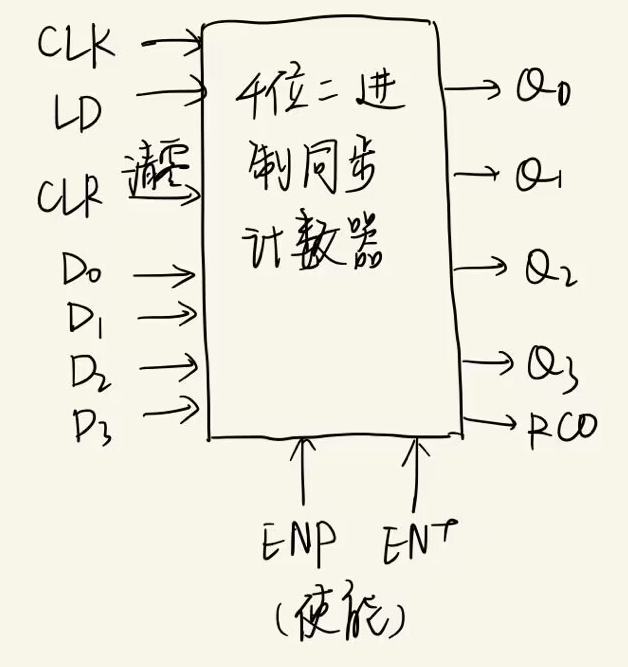
\includegraphics[width=0.8\textwidth]{1.1.png}
    \caption{4位同步二进制计数器整体方案设计}
    \end{figure}

    \subsubsection{顶层模块设计}
    实验电路较为简单,不需要顶层模块设计图。

    \subsubsection{引脚作用}
    \begin{table}[H]
    \centering
    \begin{tabular}{|c|c|}
        \hline
        CLK  & 时钟信号 \\ \hline
        LD,CLR,$D_{0}\thicksim D_{3}$ & 输入引脚 \\ \hline
        $Q_{0}\thicksim Q_{3}$,RCO   & 输出引脚 \\ \hline
        ENP,ENT   & 使能端 \\ \hline
    \end{tabular}
    \caption{4位同步二进制计数器引脚作用}
    \end{table}

    \subsubsection{原理图和电路图}
    \begin{figure}[H]
    \centering
    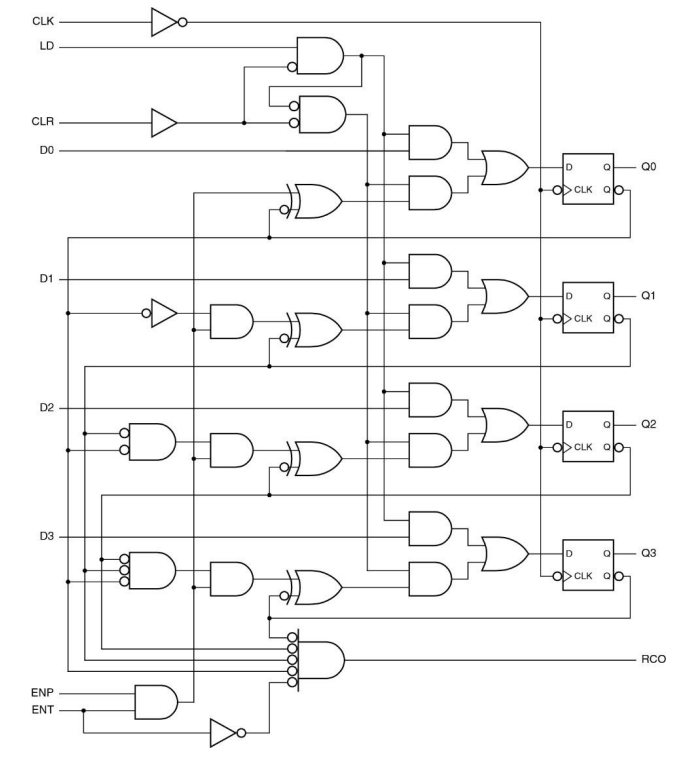
\includegraphics[width=0.8\textwidth]{1.4.1.png}
    \caption{4位同步二进制计数器原理图}
    \end{figure}

    \begin{figure}[H]
    \centering
    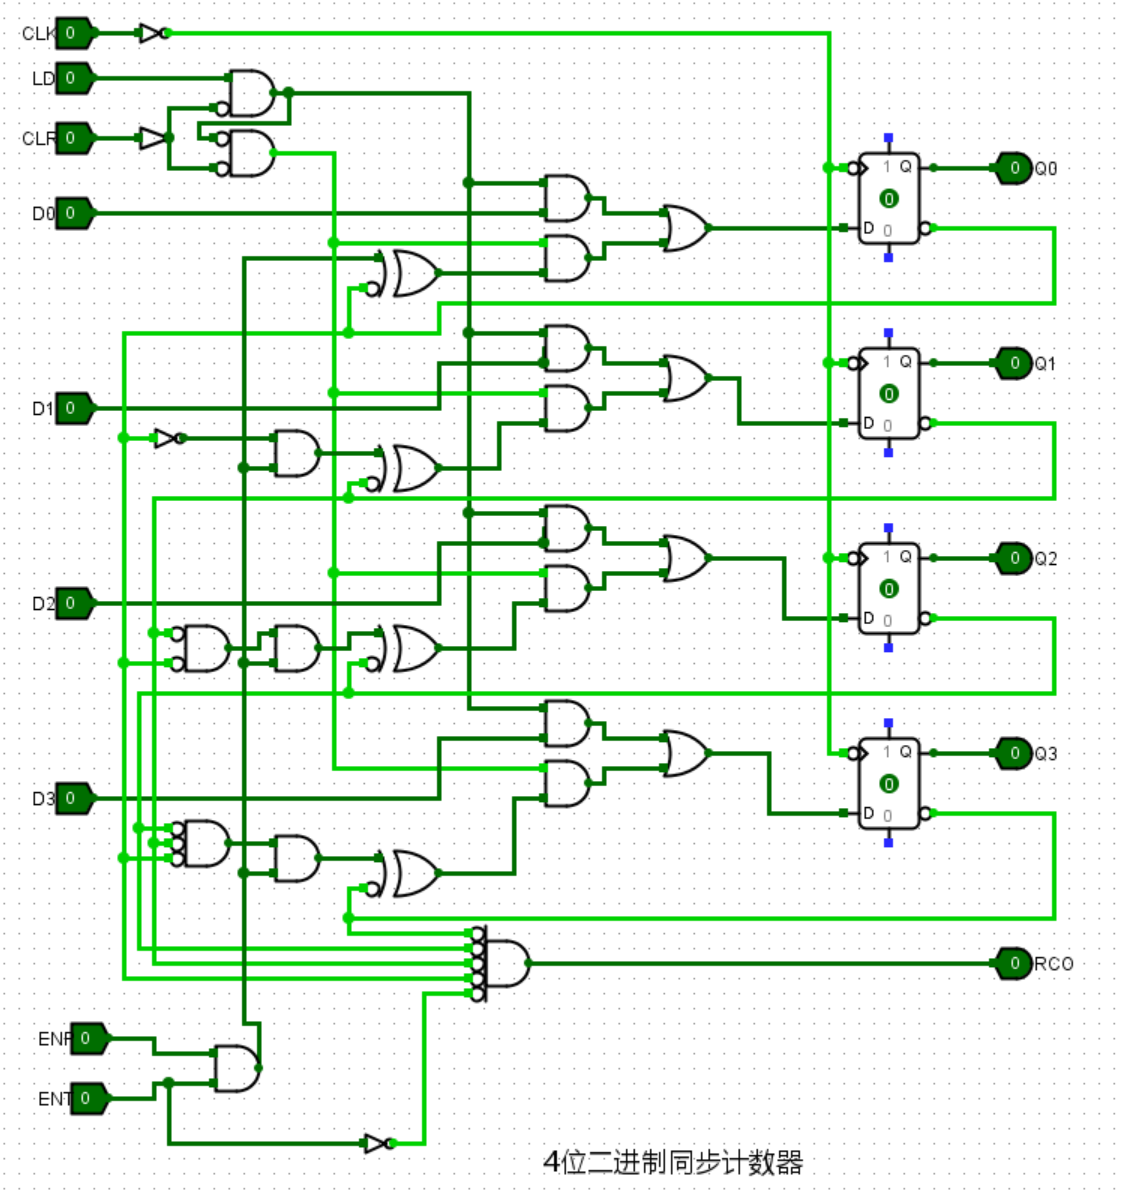
\includegraphics[width=0.8\textwidth]{1.4.2.png}
    \caption{4位同步二进制计数器电路图}
    \end{figure}

    \subsubsection{仿真测试图}
    \begin{figure}[H]
    \centering
    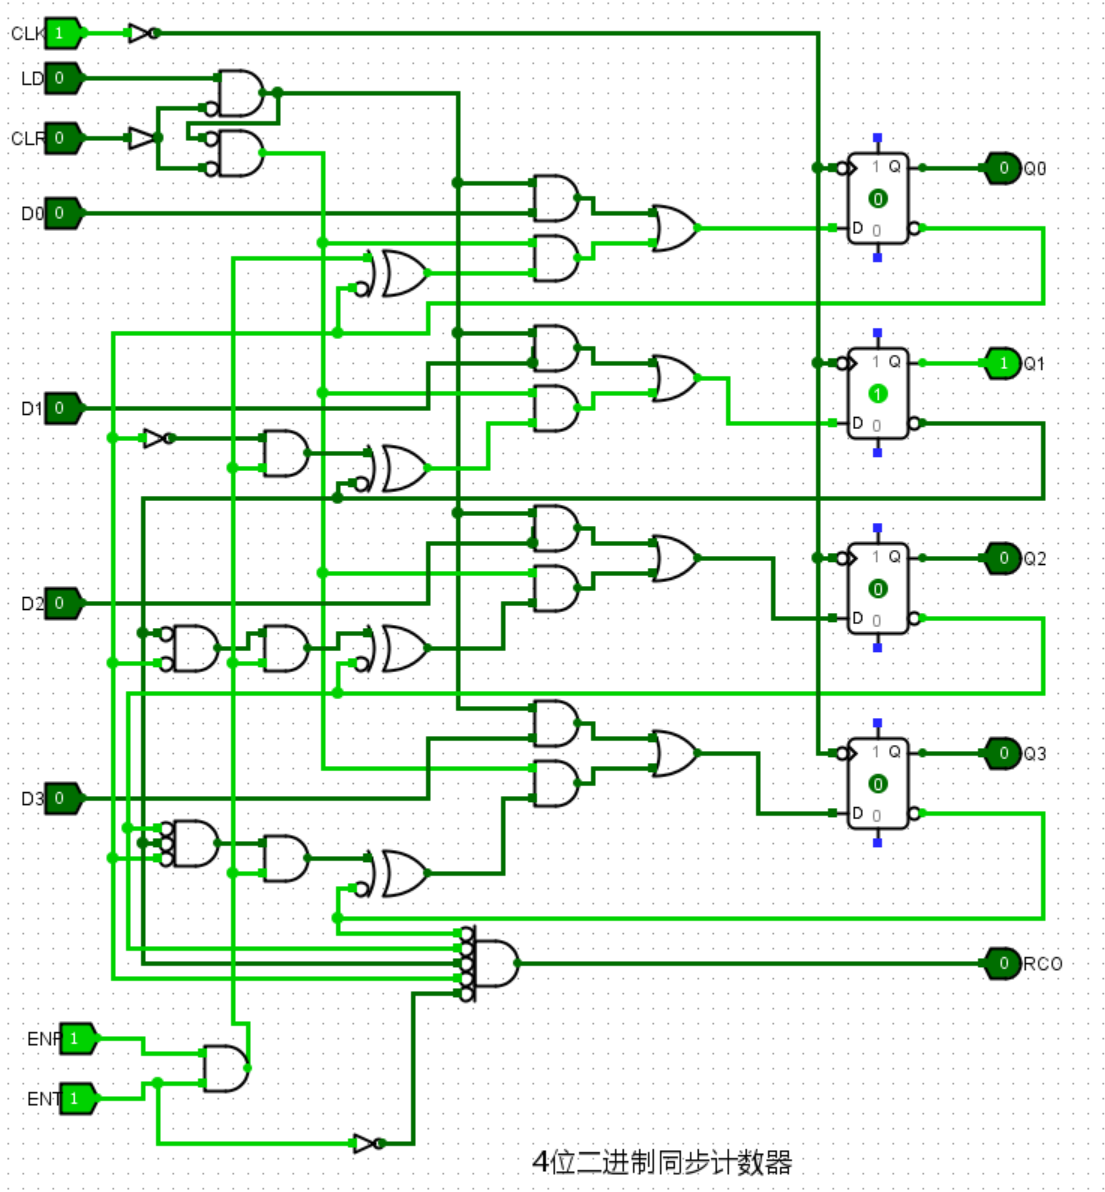
\includegraphics[width=0.4\textwidth]{1.5.1.png}
    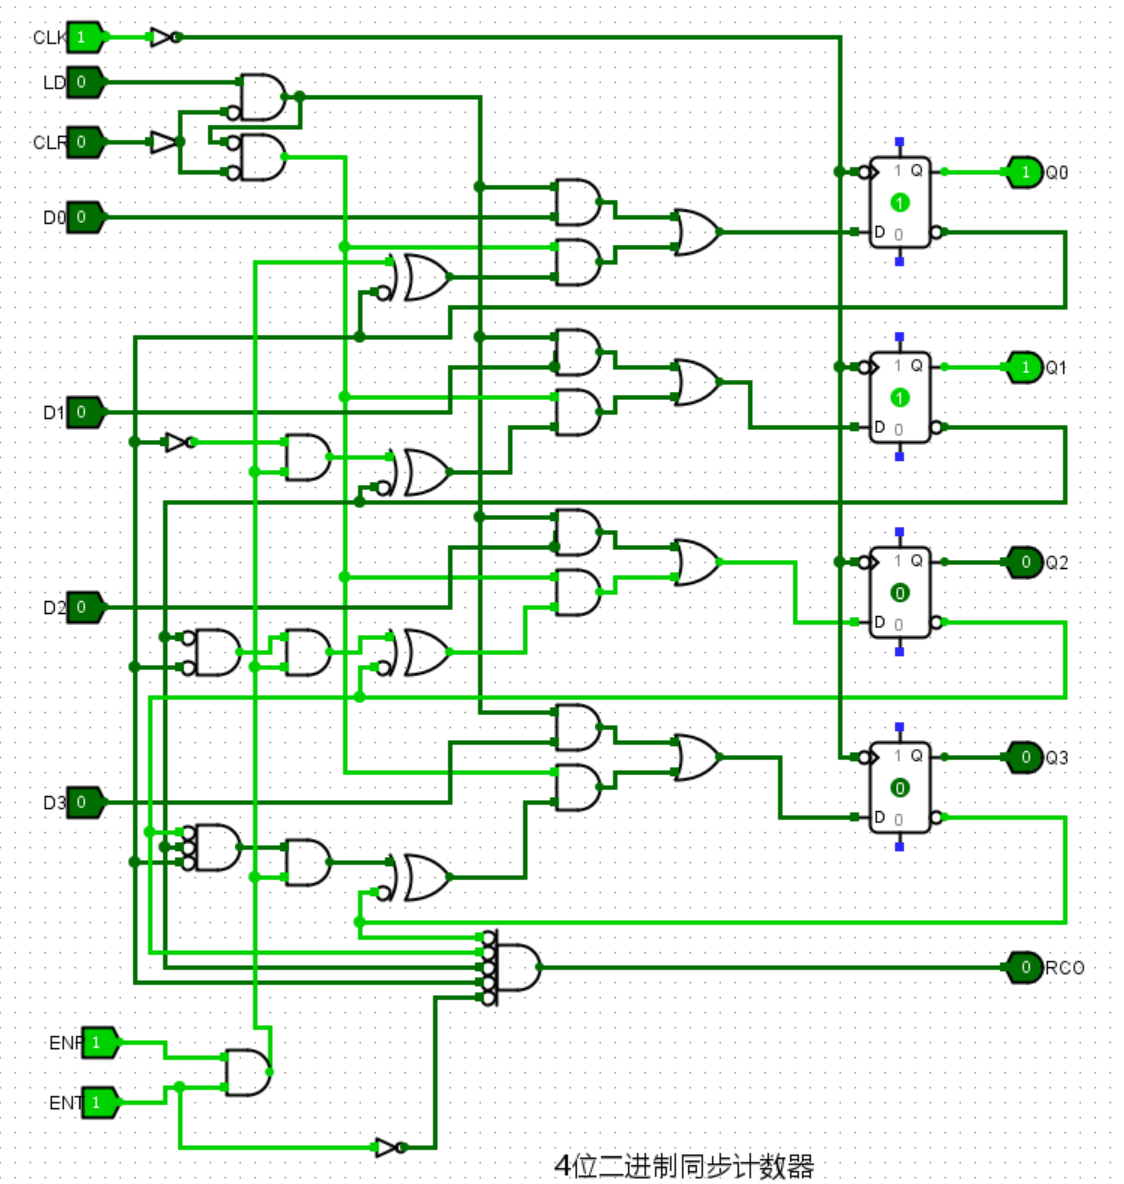
\includegraphics[width=0.4\textwidth]{1.5.2.png}
    
    \caption{4位同步二进制计数器仿真测试图}
    \end{figure}

    \begin{figure}[H]
    \centering
    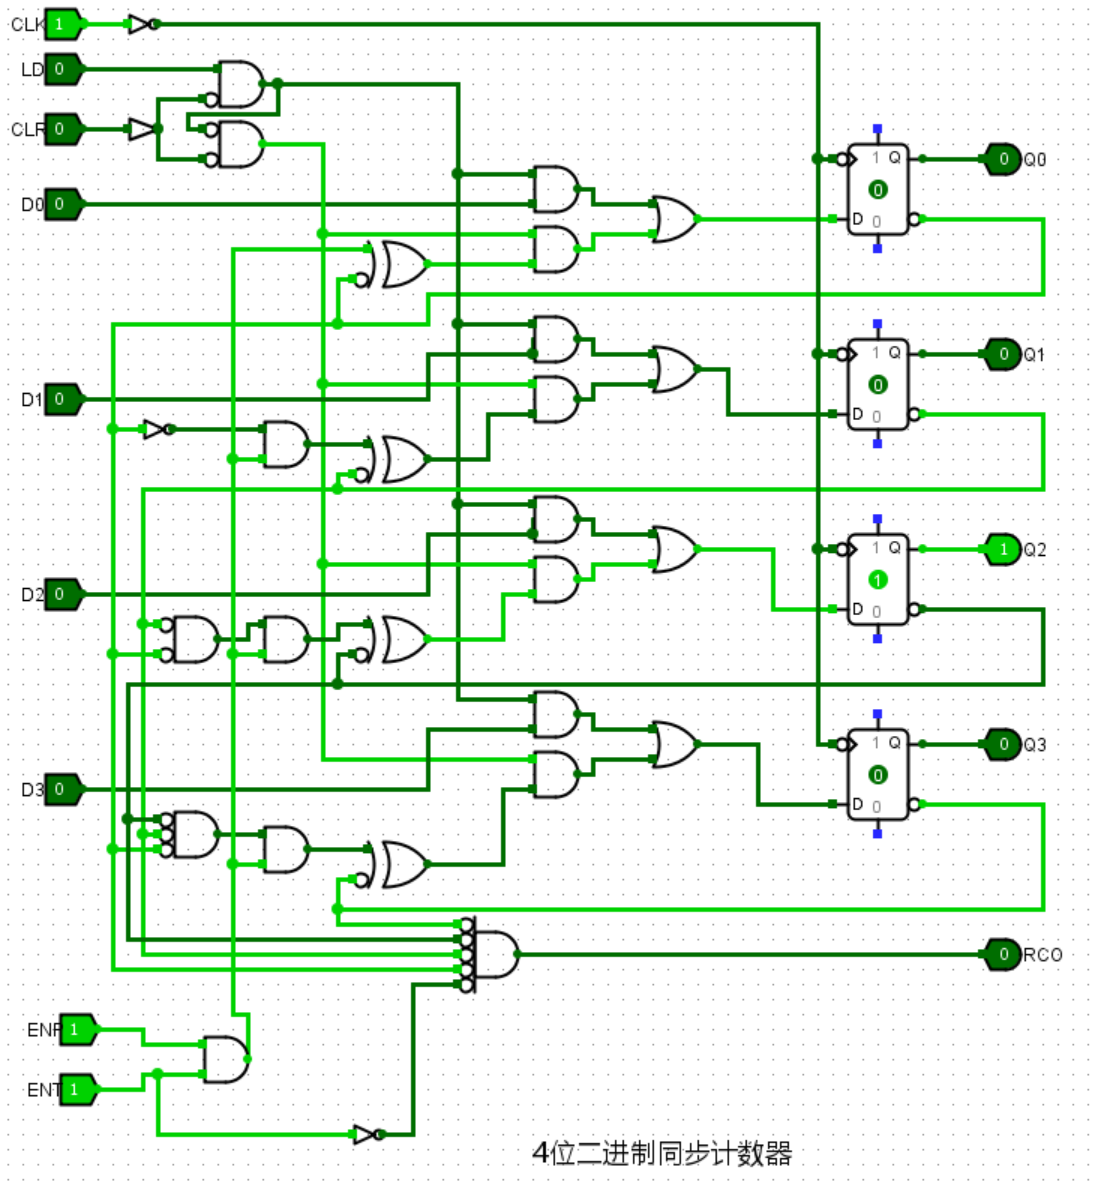
\includegraphics[width=0.4\textwidth]{1.5.3.png}  
    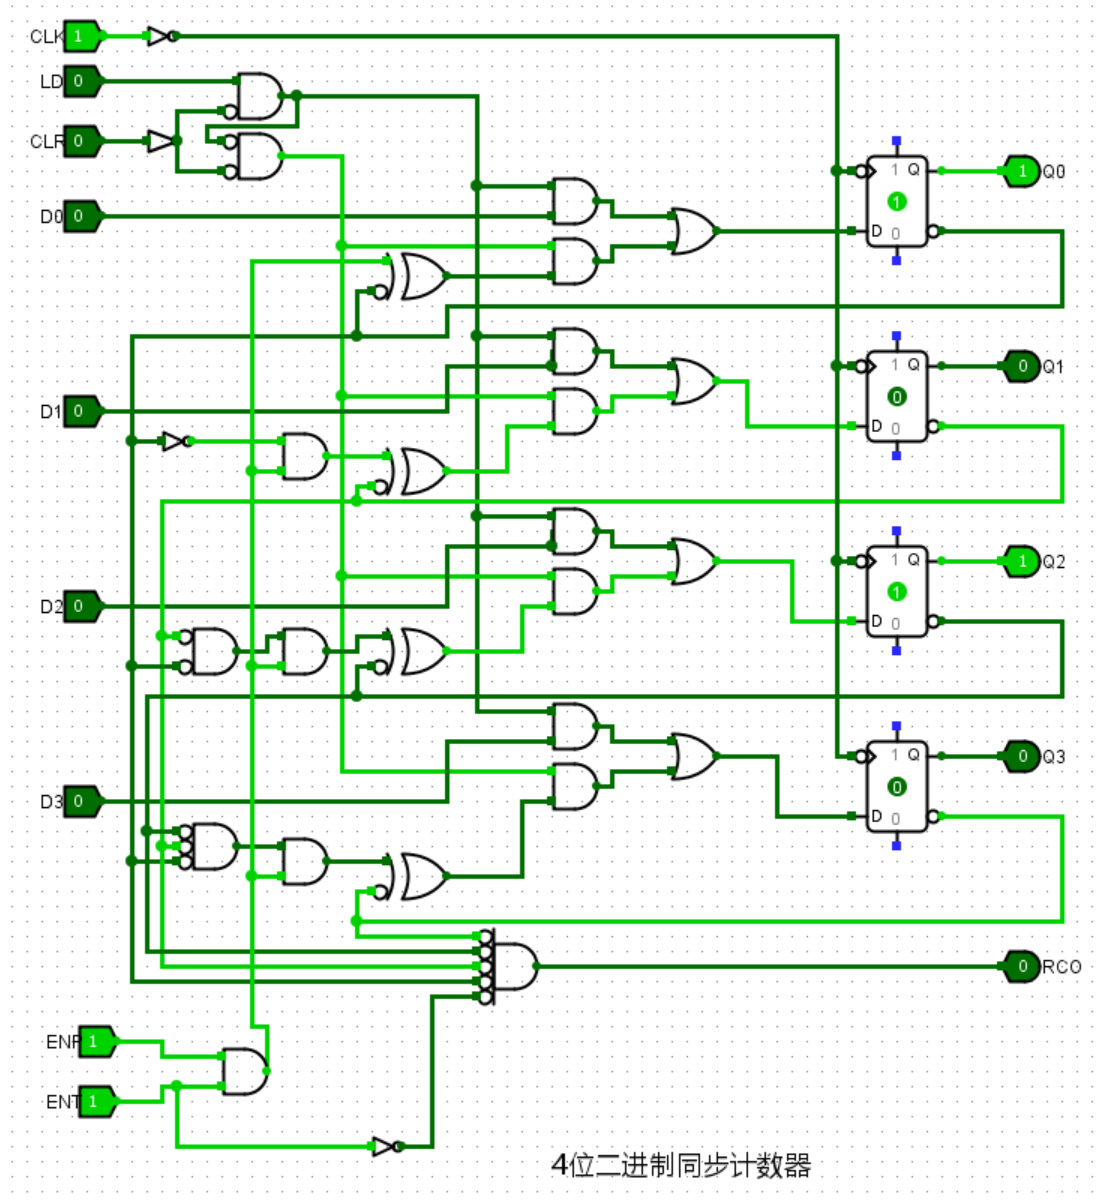
\includegraphics[width=0.4\textwidth]{1.5.4.png}
    \caption{4位同步二进制计数器仿真测试图}
    \end{figure}
    先点击CLR使得输出为置为0,在图一的初始计数器为2,经过3个时钟周期后变为5。
    
    功能表如下。
    
    \begin{table}[H]
    \centering
    \begin{tabular}{|c|c|c|}
        \hline
        Inputs & Current State & Next State \\ \hline
        CLR,LD,ENT,ENP & $Q_{3}Q_{2}Q_{1}Q_{0}$ & $Q_{3}^{*}Q_{2}^{*}Q_{1}^{*}Q_{0}^{*}$ \\ \hline
        1xxx & xxxx & 0000 \\ \hline
        01xx & xxxx & $D_{3}D_{2}D_{1}D_{0}$ \\ \hline
        000x & xxxx & $Q_{3}Q_{2}Q_{1}Q_{0}$ \\ \hline
        00x0 & xxxx & $Q_{3}Q_{2}Q_{1}Q_{0}$ \\ \hline
        0011 & 0000 & 0001 \\ \hline
        0011 & 0001 & 0010 \\ \hline
        0011 & 0010 & 0011 \\ \hline
        \multicolumn{3}{|c|}{......} \\ \hline
        0011 & 1110 & 1111 \\ \hline
        0011 & 1111 & 0000 \\ \hline
    \end{tabular}
    \caption{4位同步二进制计数器功能表}
    \end{table}

    \subsubsection{错误现象及分析}
    在完成实验的过程中,没有遇到任何错误。

    \subsection{数字时钟实验}
    \subsubsection{整体方案设计}
    \begin{figure}[H]
    \centering
    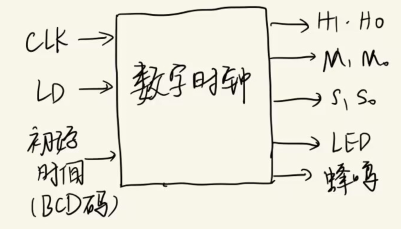
\includegraphics[width=0.8\textwidth]{2.1.png}
    \caption{数字时钟整体方案设计}
    \end{figure}

    \subsubsection{顶层模块设计}
    实验电路较为简单,不需要顶层模块设计图。

    \subsubsection{引脚作用}
    \begin{table}[H]
    \centering
    \begin{tabular}{|c|c|}
        \hline
        CLK & 时钟信号 \\ \hline
        LD,时/分/秒高/低位 & 输入引脚 \\ \hline
        LED,$H_{1},H_{0},M_{1},M_{0},S_{1},S_{0}$,蜂鸣使能  & 输出引脚 \\ \hline
    \end{tabular}
    \caption{数字时钟引脚作用}
    \end{table}
    
    \subsubsection{原理图和电路图}
    \begin{figure}[H]
    \centering
    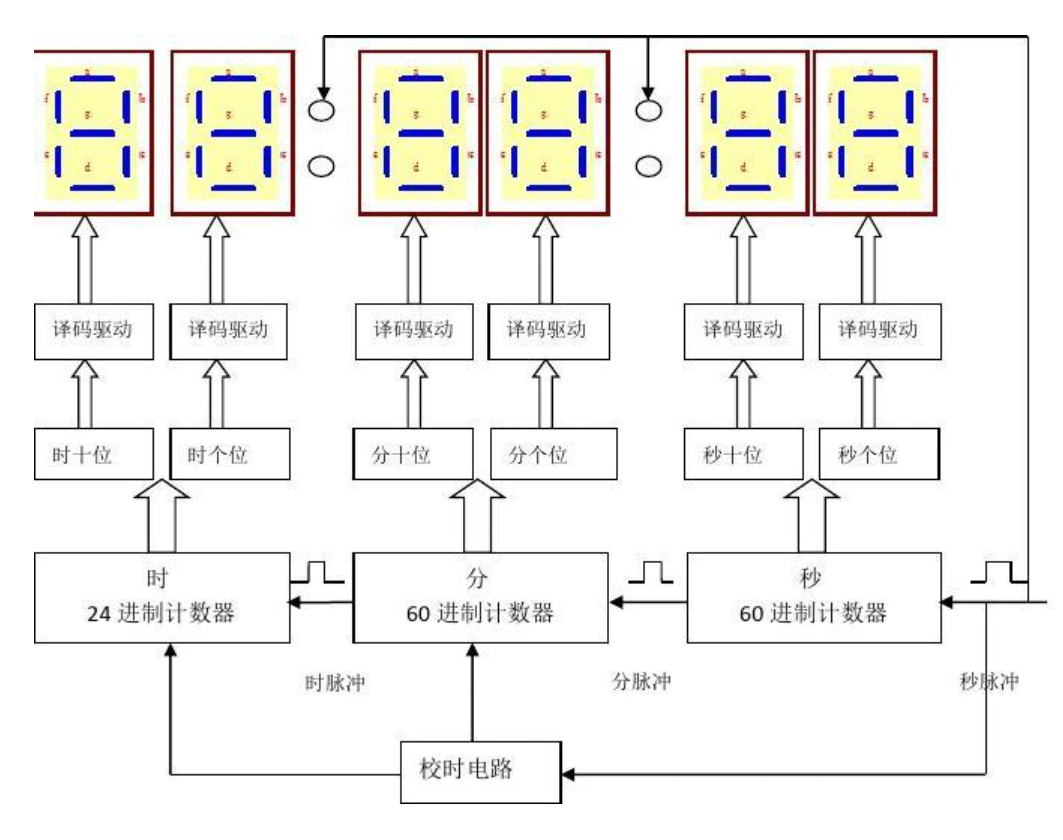
\includegraphics[width=0.8\textwidth]{2.4.1.png}

    \caption{数字时钟原理图}
    \end{figure}

    \begin{figure}[H]
    \centering
    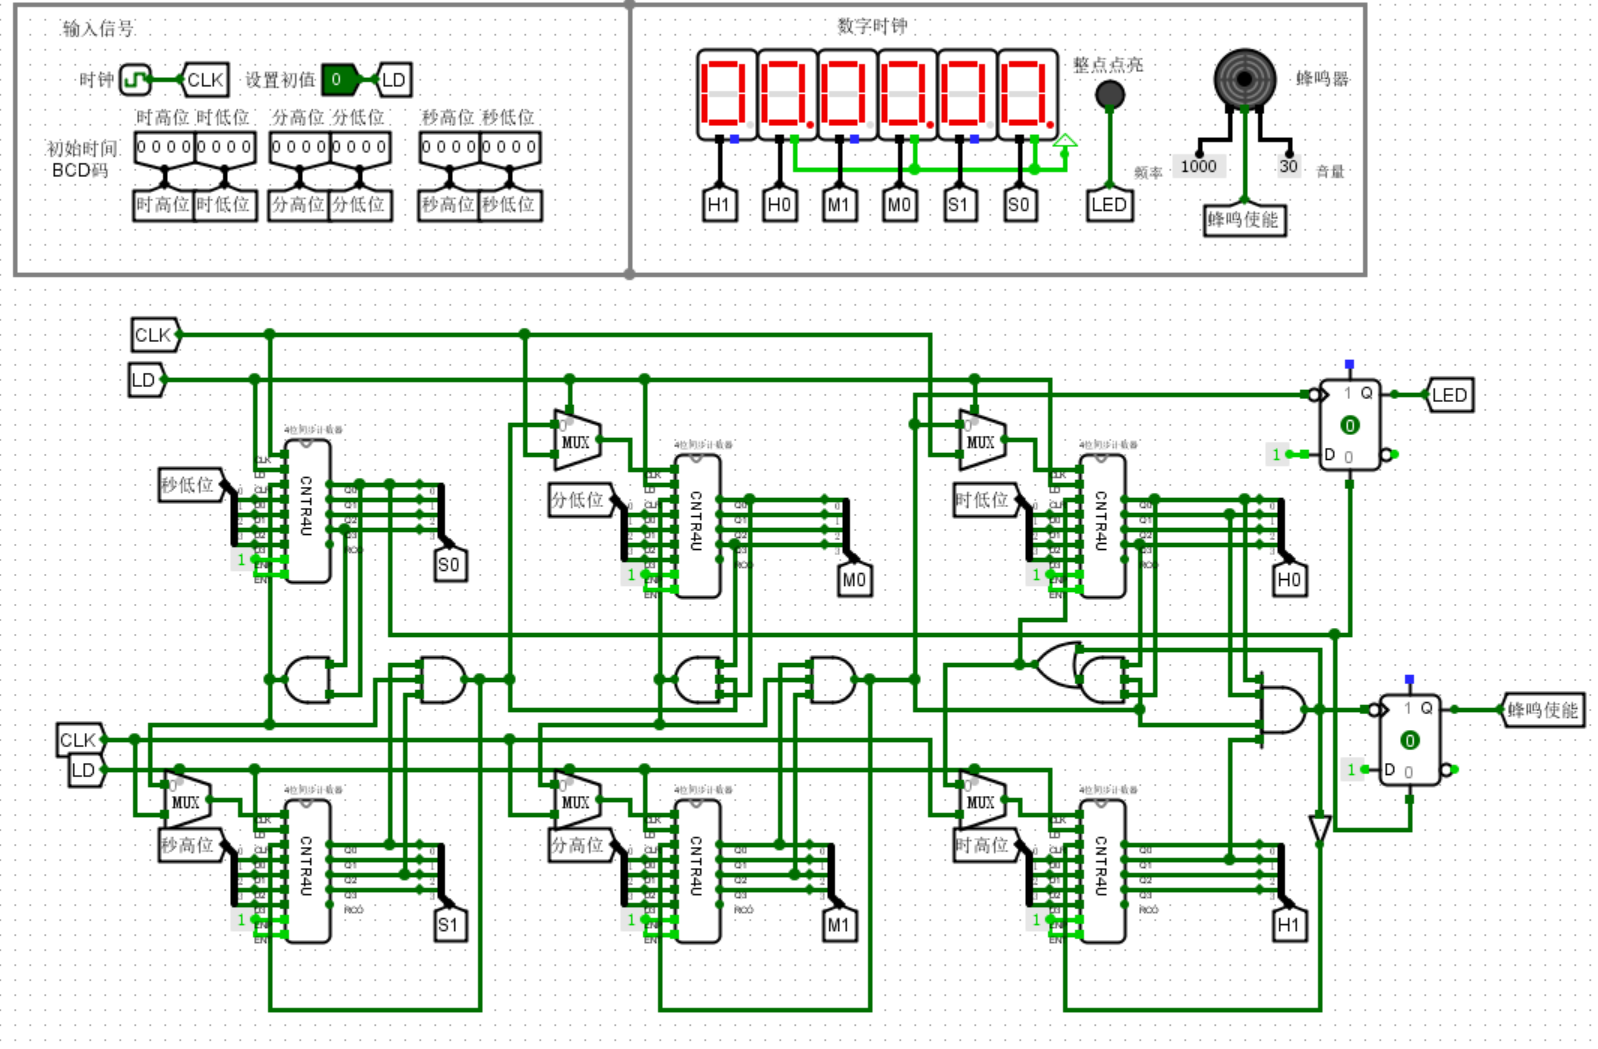
\includegraphics[width=0.8\textwidth]{2.4.2.png}
    \caption{数字时钟电路图}
    \end{figure}

    \subsubsection{仿真测试图}
    \begin{figure}[H]
    \centering
    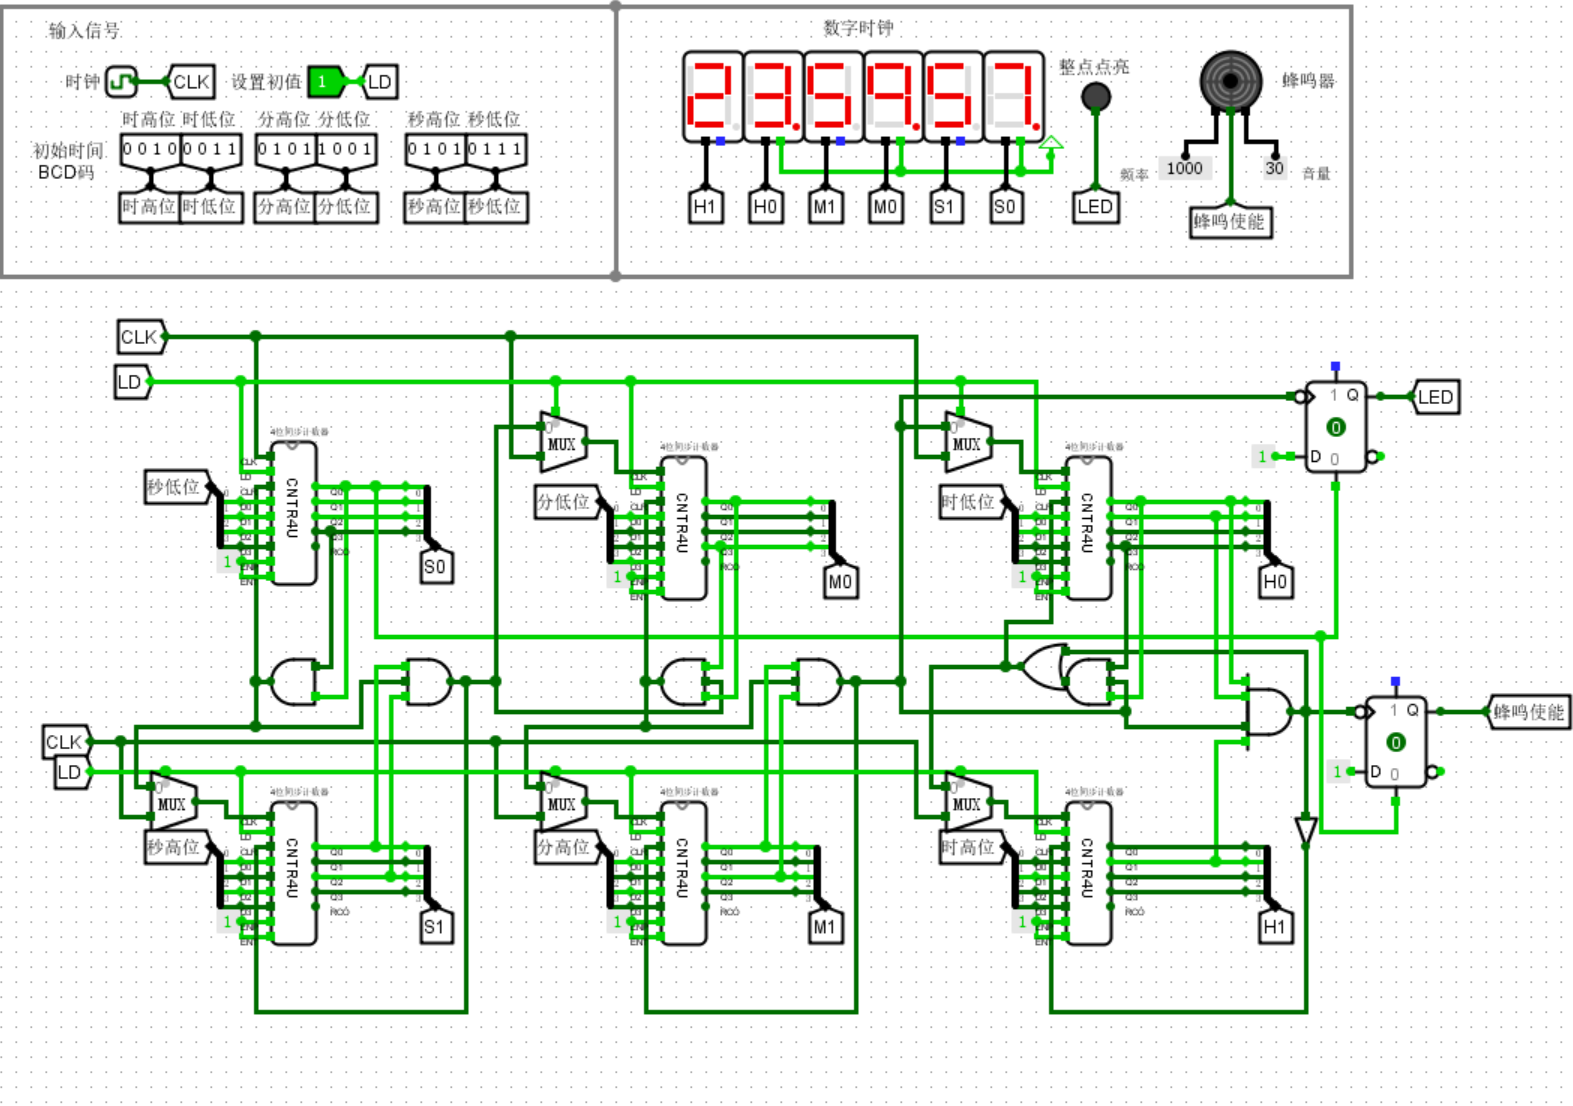
\includegraphics[width=0.8\textwidth]{2.5.1.png}
    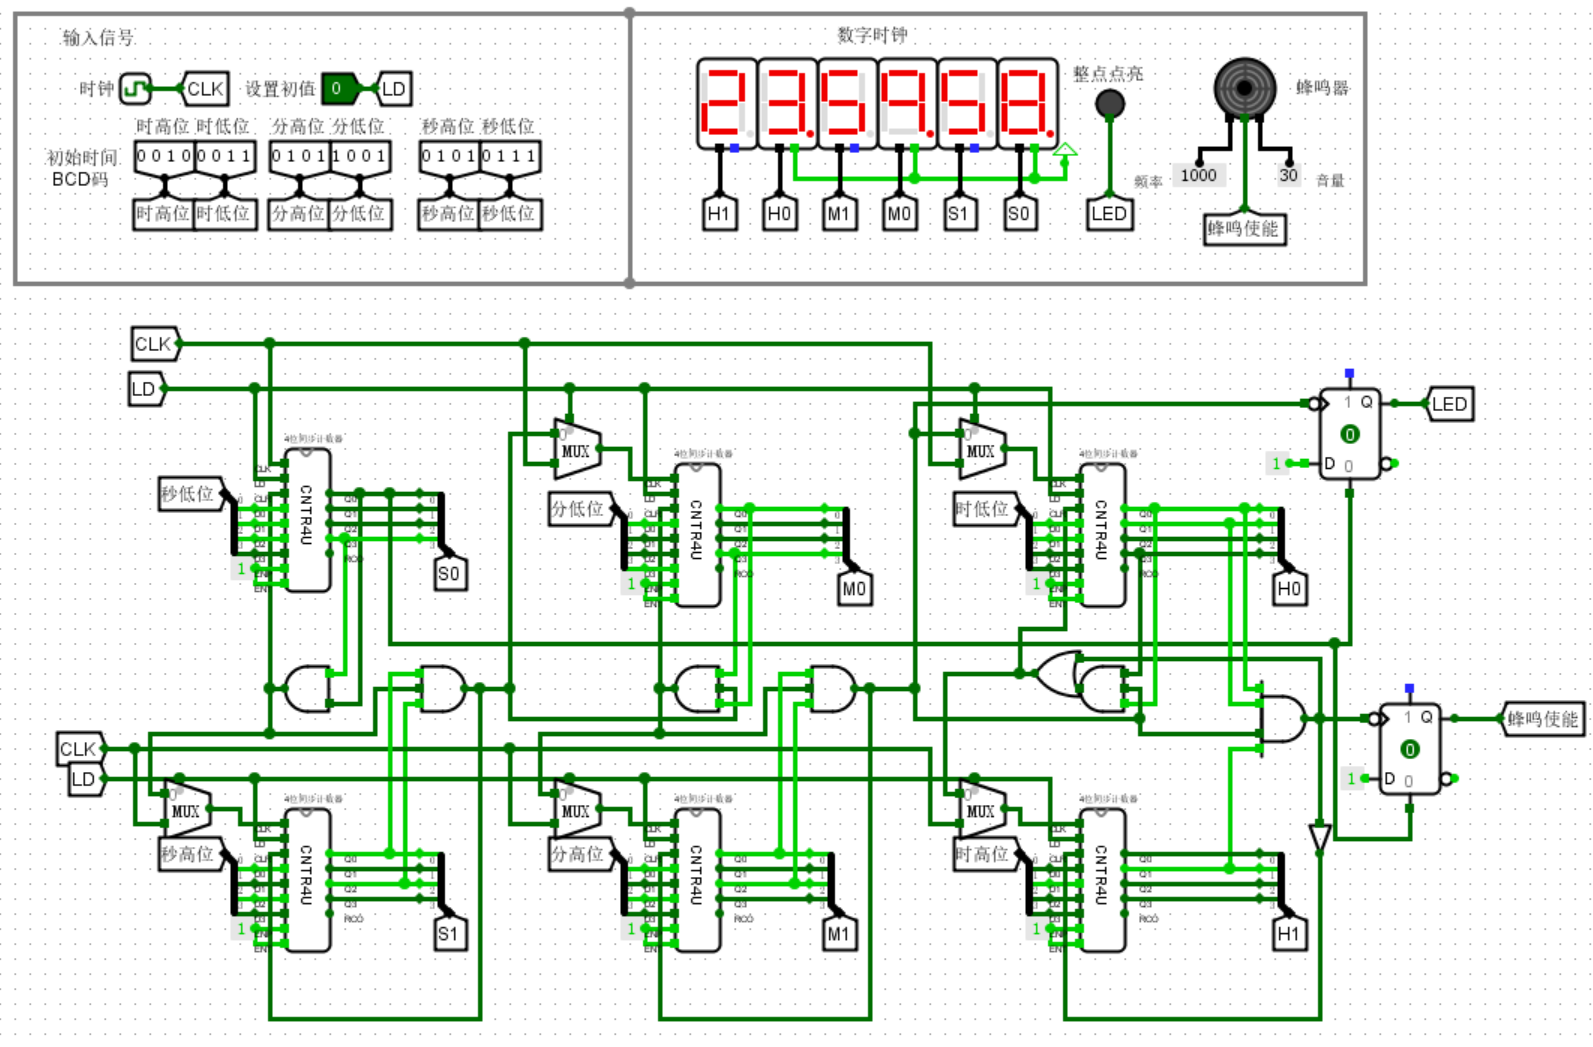
\includegraphics[width=0.8\textwidth]{2.5.2.png}
    \caption{数字时钟仿真测试图}
    \end{figure}
    
    \begin{figure}[H]
    \centering
    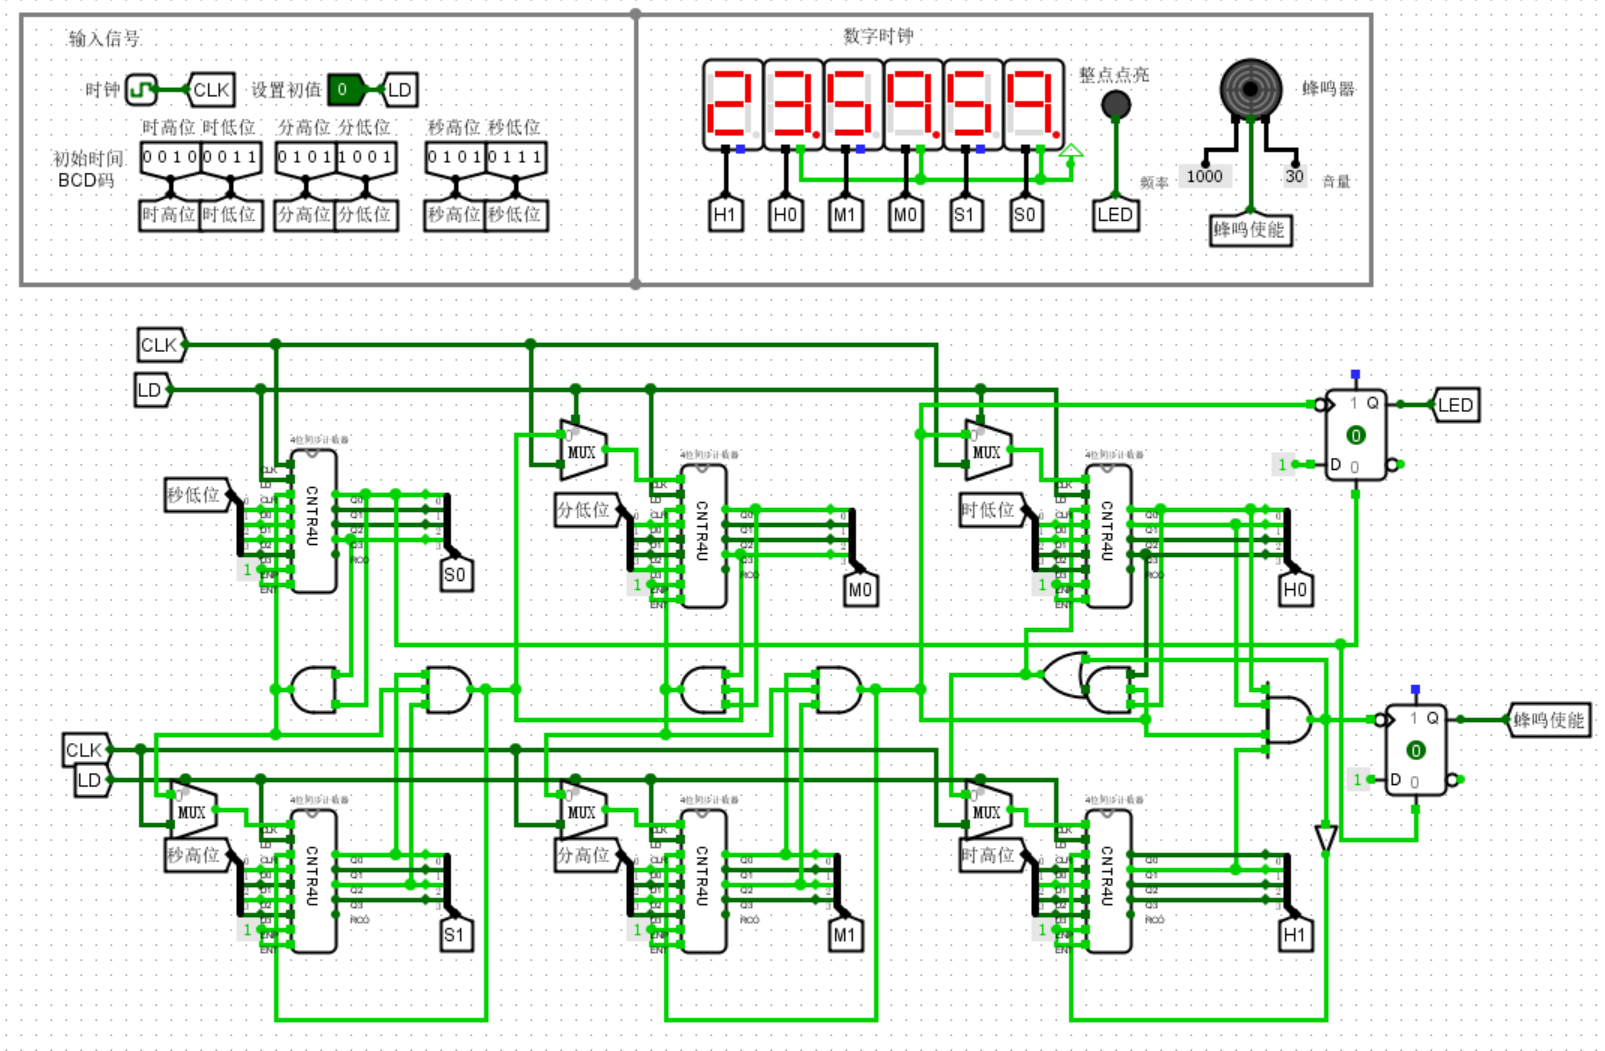
\includegraphics[width=0.8\textwidth]{2.5.3.png}
    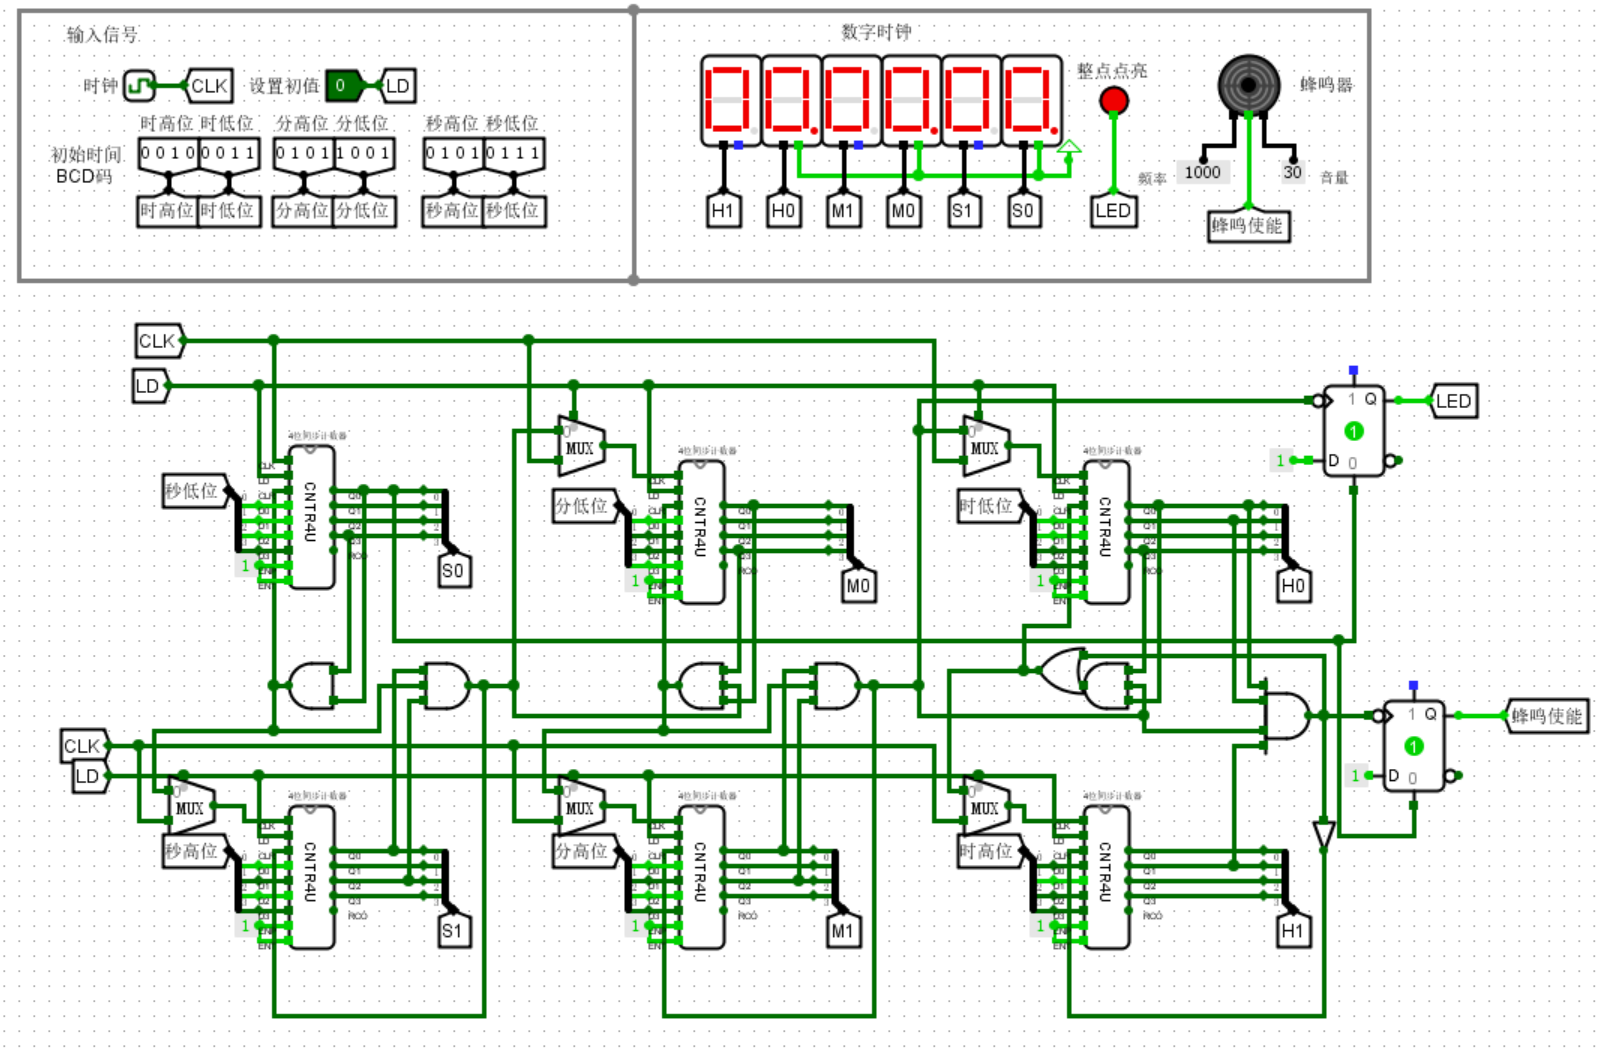
\includegraphics[width=0.8\textwidth]{2.5.4.png}
    \caption{数字时钟仿真测试图}
    \end{figure}
    开启自动仿真和时钟连续后,设置初始为23时59分57秒,经过3秒后变为0时0分0秒,LED 灯点亮且蜂鸣器响。

    \subsubsection{错误现象及分析}
    在完成实验的过程中,没有遇到任何错误。

    \subsection{移位寄存器实验}
    \subsubsection{整体方案设计}
    \begin{figure}[H]
    \centering
    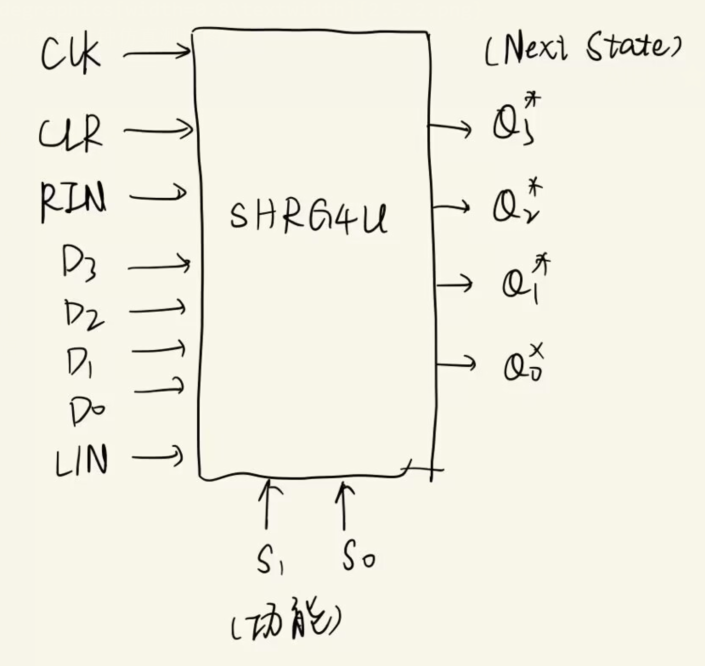
\includegraphics[width=0.8\textwidth]{3.1.png}
    \caption{移位寄存器整体方案设计}
    \end{figure}

    \subsubsection{顶层模块设计}
    实验电路较为简单,不需要顶层模块设计图。

    \subsubsection{引脚作用}
    \begin{table}[H]
    \centering
    \begin{tabular}{|c|c|}
        \hline
        CLK & 时钟信号 \\ \hline
        CLR & 清零 \\ \hline
        RIN,$D_{3},D_{2},D_{1},D_{0},S_{1},S_{0},LIN$ & 输入引脚 \\ \hline
        $Q_{3},Q_{2},Q_{1},Q_{0}$ & 输出引脚 \\ \hline
    \end{tabular}
    \caption{移位寄存器引脚作用}
    \end{table}

    \subsubsection{原理图和电路图}
    \begin{figure}[H]
    \centering
    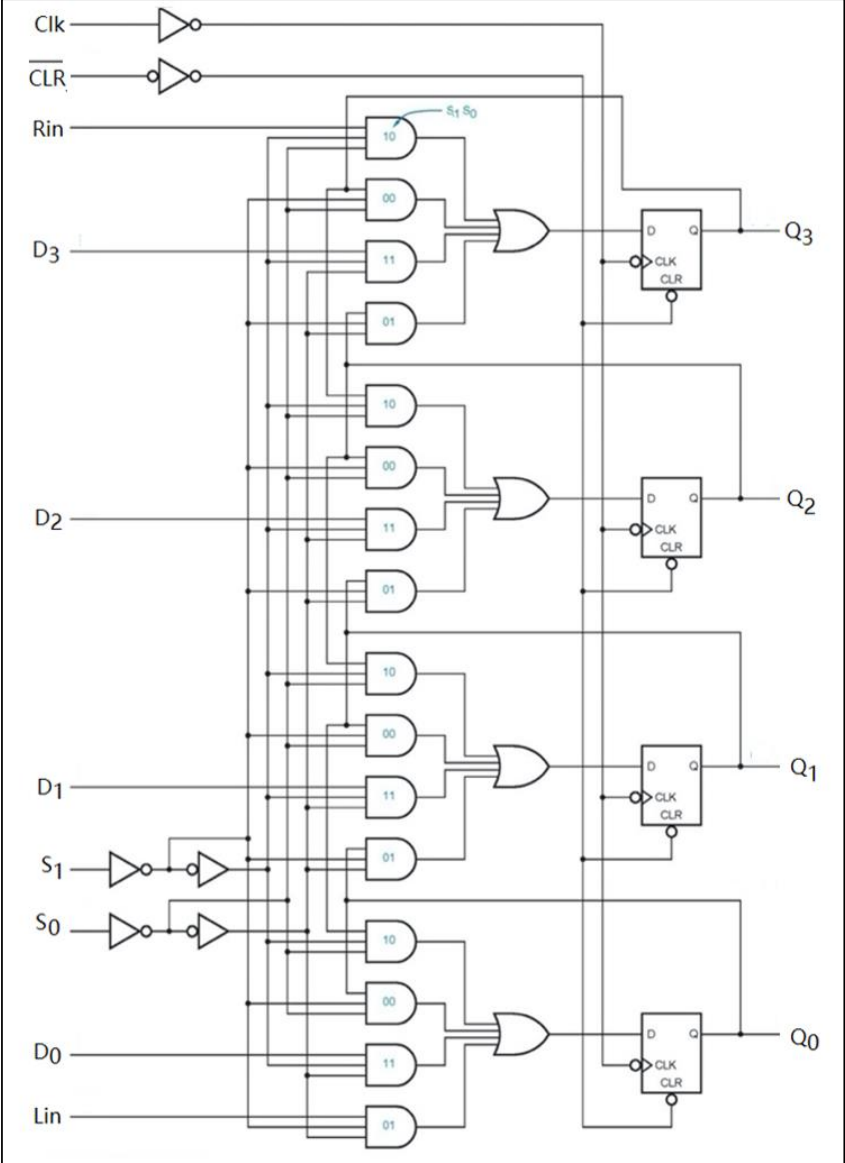
\includegraphics[width=0.8\textwidth]{3.4.1.png}
    \caption{移位寄存器原理图}
    \end{figure}    

    \begin{figure}[H]
    \centering
    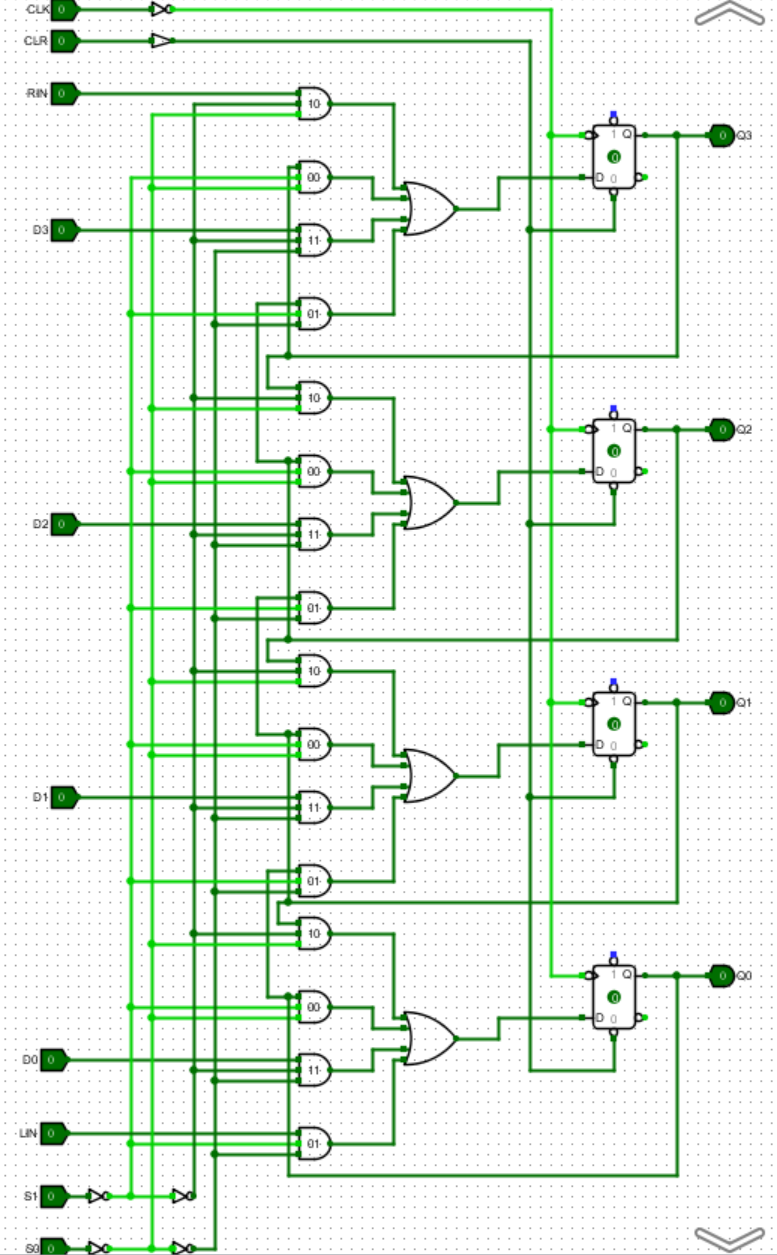
\includegraphics[width=0.8\textwidth]{3.4.2.png}
    \caption{移位寄存器电路图}
    \end{figure}

    \subsubsection{仿真测试图}
    \begin{figure}[H]
    \centering
    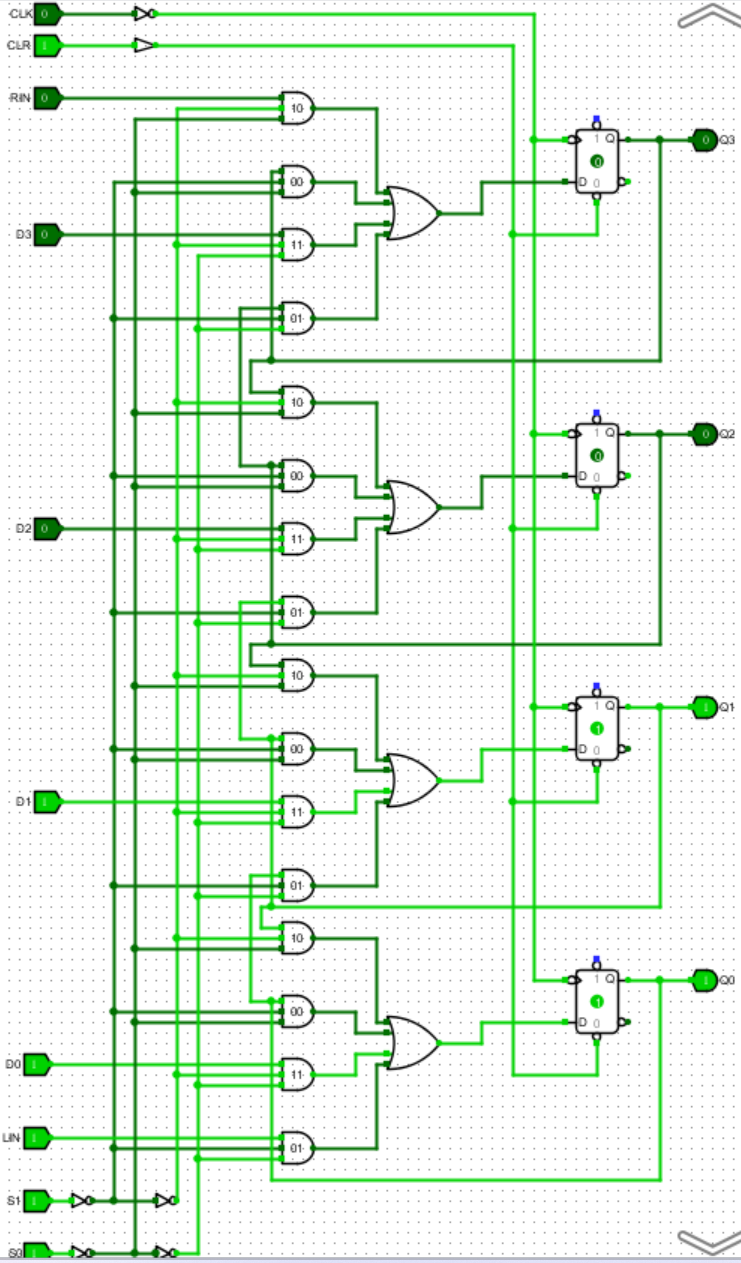
\includegraphics[width=0.8\textwidth]{3.5.1.png}
    \caption{移位寄存器仿真测试图}
    \end{figure}

    \begin{figure}[H]
    \centering
    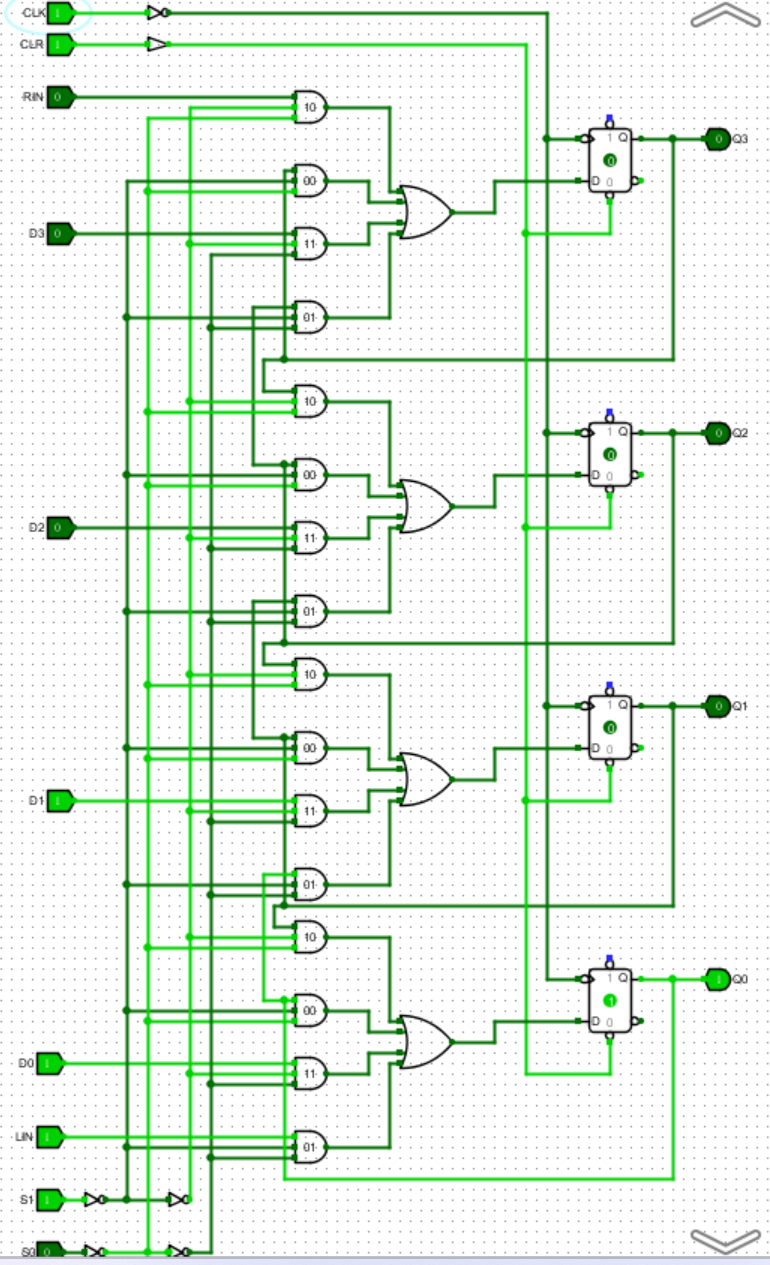
\includegraphics[width=0.8\textwidth]{3.5.2.png}
    \caption{移位寄存器仿真测试图}
    \end{figure}
    
    \begin{figure}[H]
    \centering






    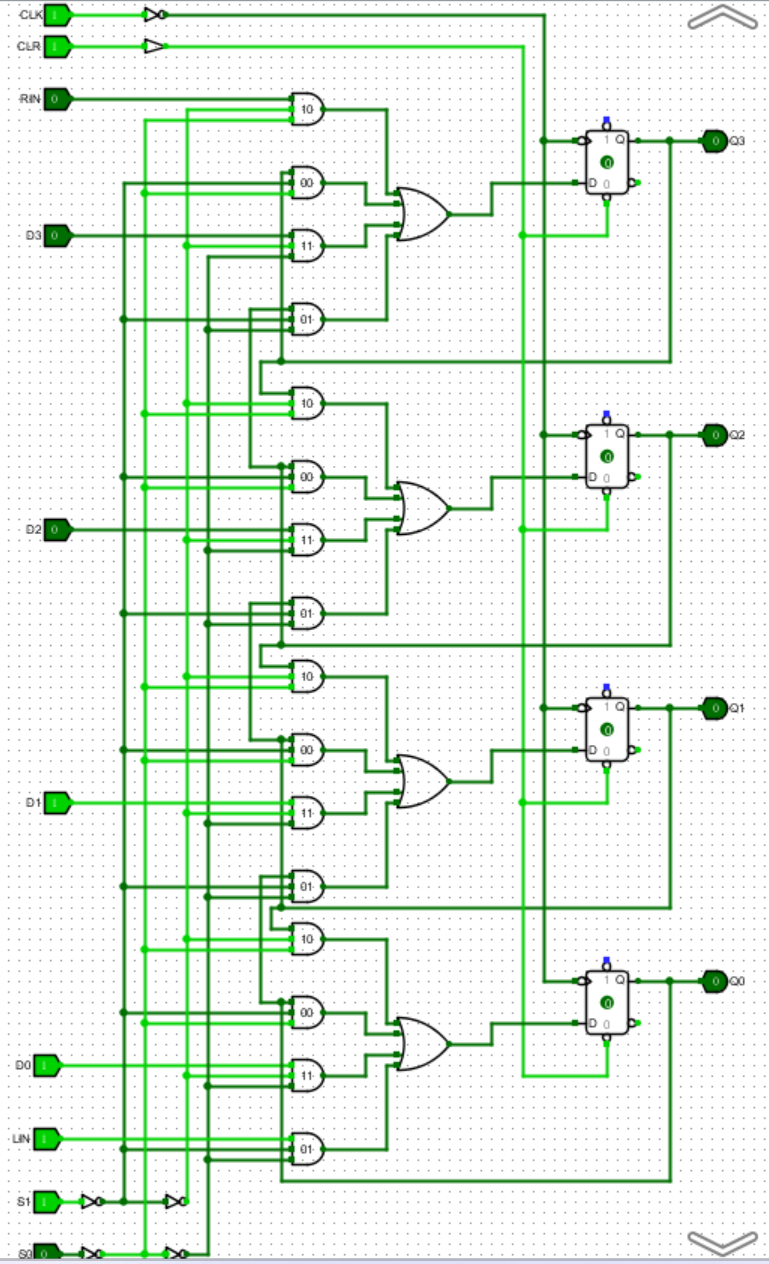
\includegraphics[width=0.8\textwidth]{3.5.3.png}
    \caption{移位寄存器仿真测试图}
    \end{figure}

    \begin{figure}[H]
    \centering
    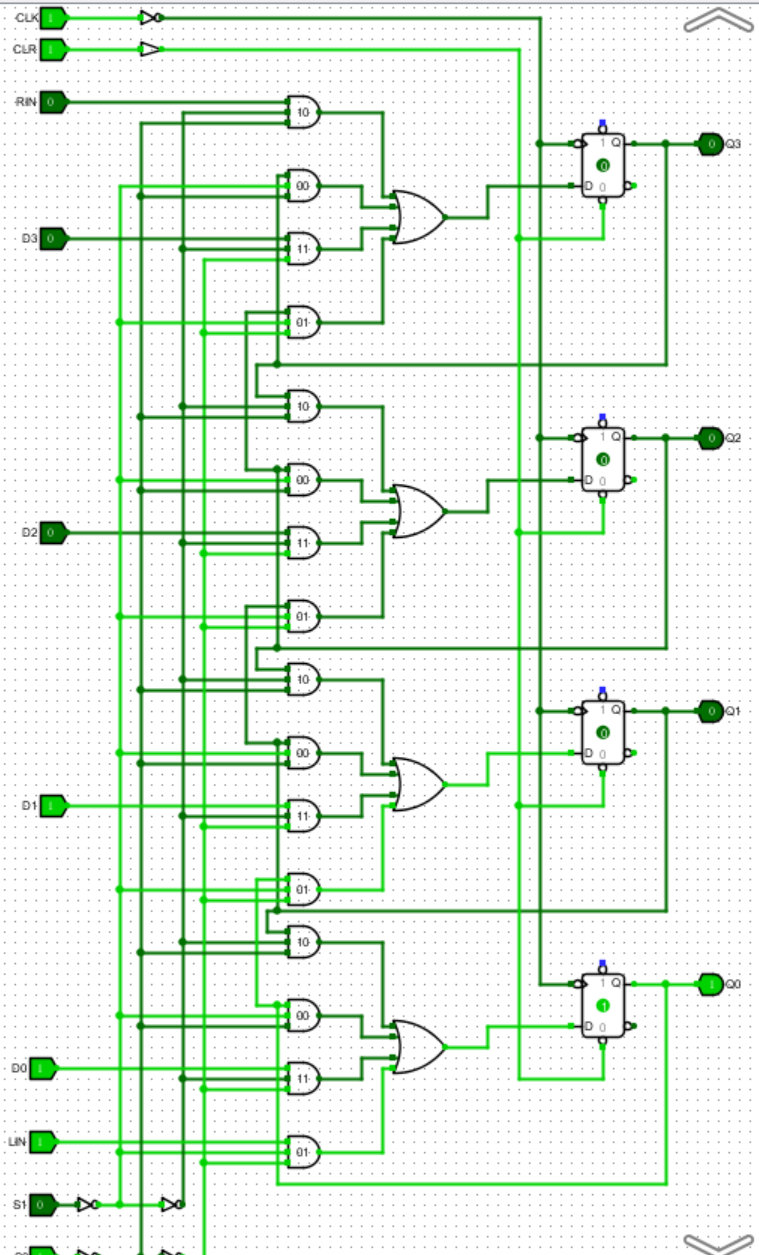
\includegraphics[width=0.8\textwidth]{3.5.4.png}
    \caption{移位寄存器仿真测试图}
    \end{figure}

    设置RIN为0,LIN为0,CLR为1,初始值为0011,$S_{1}S_{0}$为11进行装载,然后使$S_{1}S_{0}$为10(右移),经过两个时钟周期数值分别变为0001、0000,再将$S_{1}S_{0}$变为01(左移),经过一个时钟周期数值分别变为0001。

    功能表如下。
    \begin{table}[H]
    \centering
    \begin{tabular}{|c|c|c|c|c|c|c|c|}
        \hline
        \multirow{2}{*}{功能}
        & \multicolumn{3}{c|}{输入} & \multicolumn{4}{c|}{下一个状态} \\ \cline{2-8}
        & CLR & $S_{1}$ & $S_{0}$ & $Q_{3}^{*}$ & $Q_{2}^{*}$ & $Q_{1}^{*}$ & $Q_{0}^{*}$ \\ 
        \hline
        \multirow{1}{*}{清零} & 0 & x & x & 0 & 0 & 0 & 0 \\ \hline
        \multirow{1}{*}{保持} & 1 & 0 & 0 & $Q_{3}$ & $Q_{2}$ & $Q_{1}$ & $Q_{0}$ \\ \hline
        \multirow{1}{*}{右移} & 1 & 1 & 0 & RIN & $Q_{3}$ & $Q_{2}$ & $Q_{1}$ \\ \hline
        \multirow{1}{*}{左移} & 1 & 0 & 1 & $Q_{2}$ & $Q_{1}$ & $Q_{0}$ & LIN \\ \hline
        \multirow{1}{*}{装载} & 1 & 1 & 1 & $D_{3}$ & $D_{2}$ & $D_{1}$ & $D_{0}$ \\ \hline
    \end{tabular}
    \caption{移位寄存器功能表}
    \end{table}


    \subsubsection{错误现象及分析}
    在完成实验的过程中,没有遇到任何错误。

    \subsection{4位无符号数乘法器}
    \subsubsection{整体方案设计}
    \begin{figure}[H]
    \centering
    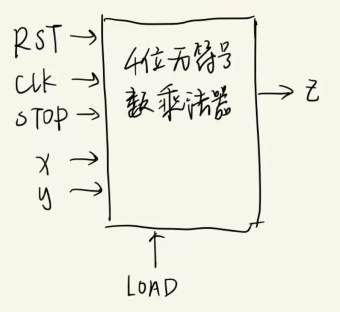
\includegraphics[width=0.8\textwidth]{4.1.png}
    \caption{4位无符号数乘法器整体方案设计}
    \end{figure}

    \subsubsection{顶层模块设计}
    实验电路较为简单,不需要顶层模块设计图。

    \subsubsection{引脚作用}
    \begin{table}[H]
    \centering
    \begin{tabular}{|c|c|}
        \hline
        CLK & 时钟信号 \\ \hline
        RST & 复位 \\ \hline
        x,y & 输入引脚 \\ \hline
        z & 输出引脚 \\ \hline
    \end{tabular}
    \caption{4位无符号数乘法器引脚作用}
    \end{table}

    \subsubsection{原理图和电路图}
    \begin{figure}[H]
    \centering
    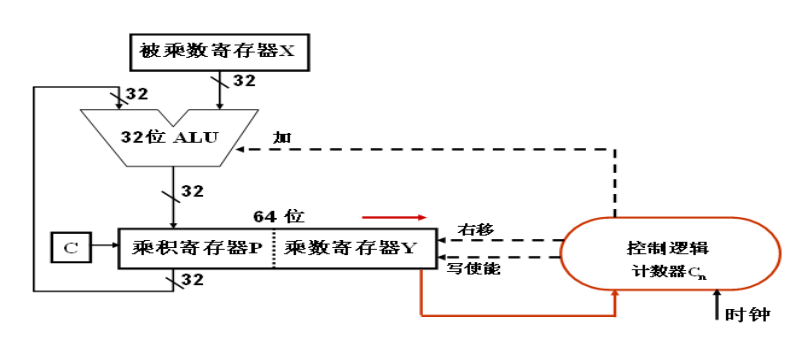
\includegraphics[width=0.8\textwidth]{4.4.1.png}
    \caption{4位无符号数乘法器原理图}
    \end{figure}

    \begin{figure}[H]
    \centering
    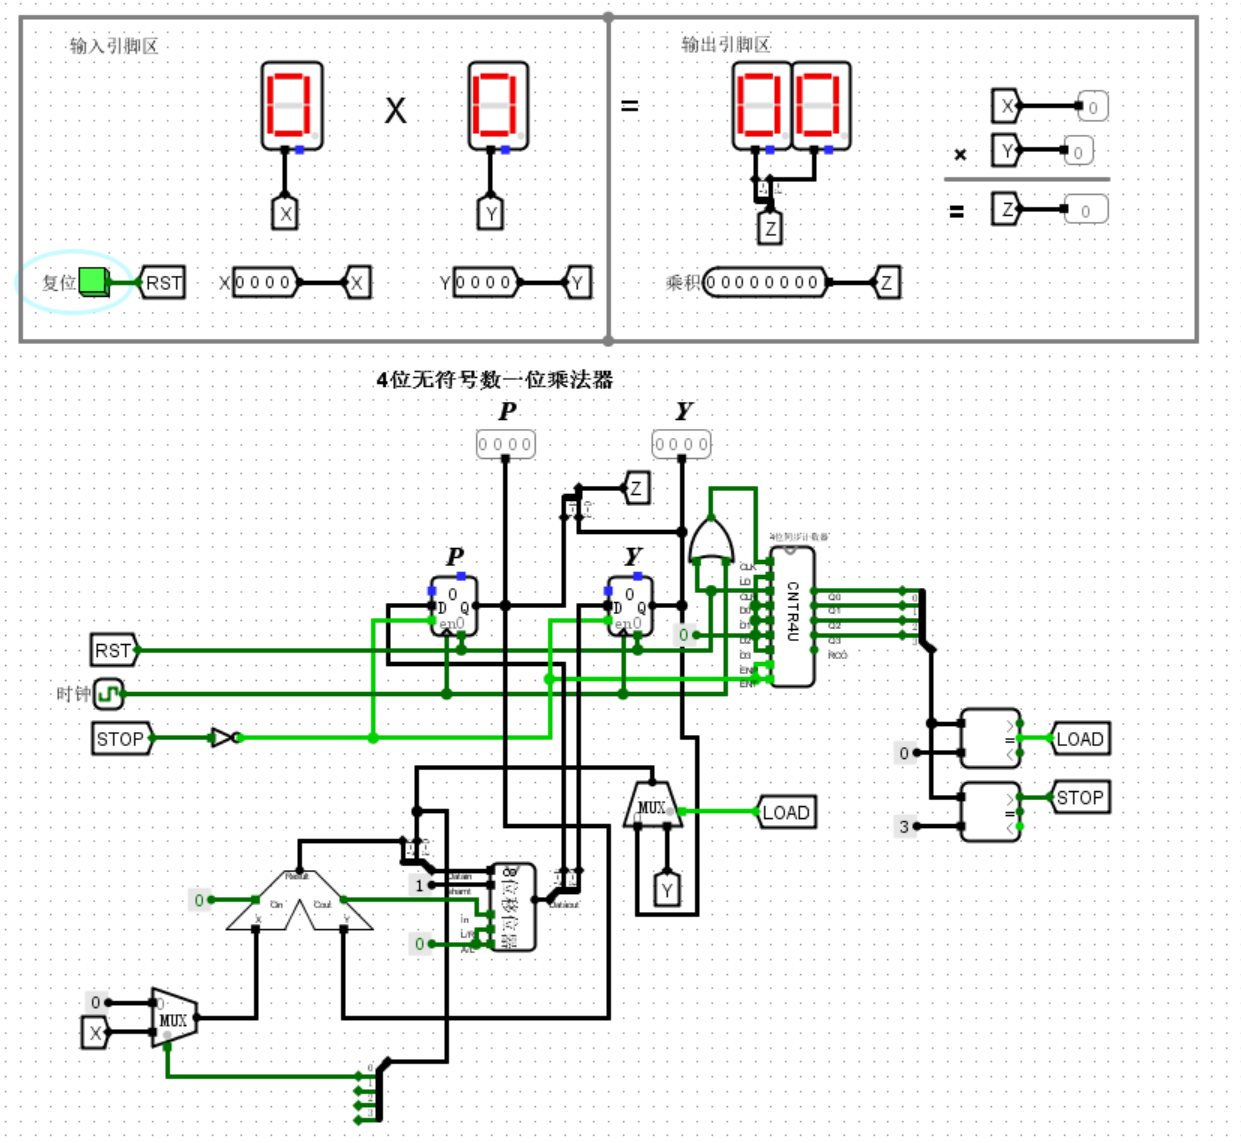
\includegraphics[width=0.8\textwidth]{4.4.2.png}
    \caption{4位无符号数乘法器电路图}
    \end{figure}

    \subsubsection{仿真测试图}
    \begin{figure}[H]
    \centering
    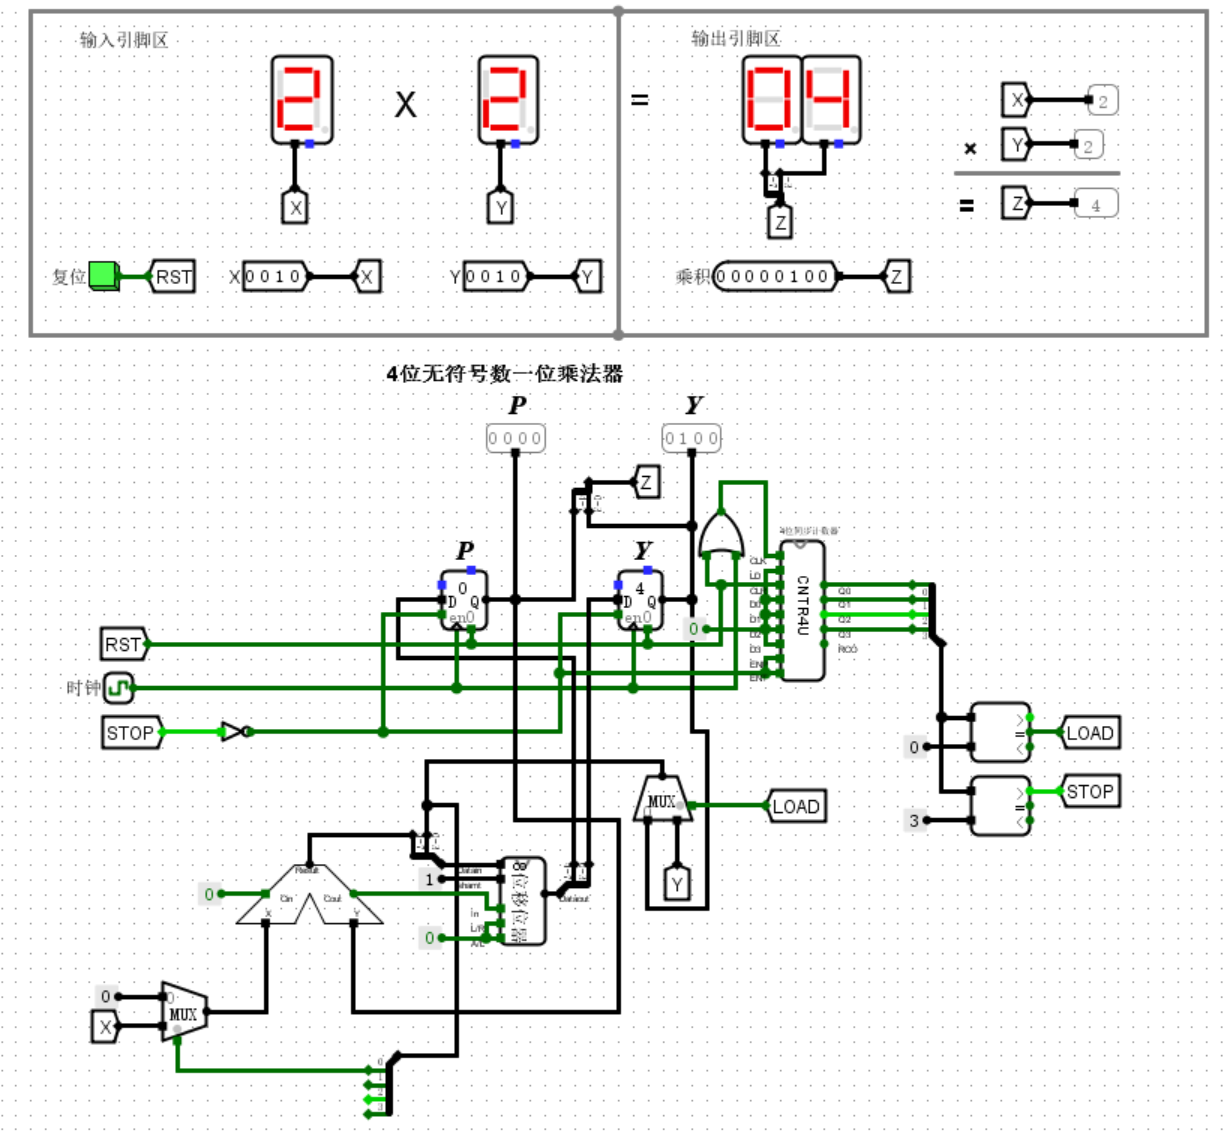
\includegraphics[width=0.7\textwidth]{4.5.1.png}
    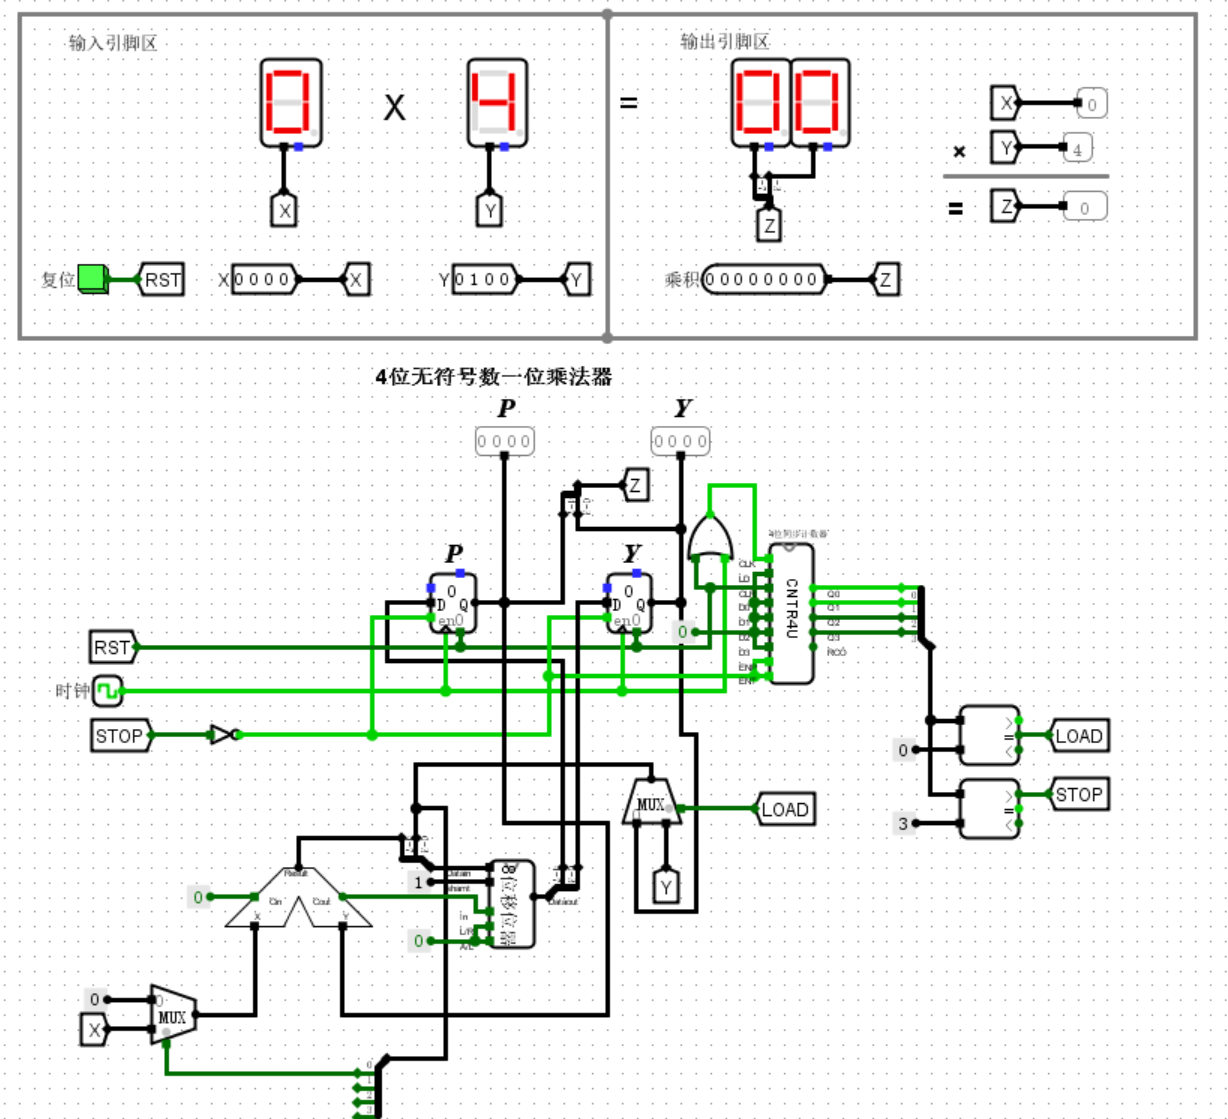
\includegraphics[width=0.7\textwidth]{4.5.2.png}
    \caption{4位无符号数乘法器仿真测试图}
    \end{figure}

    \begin{figure}[H]
    \centering
    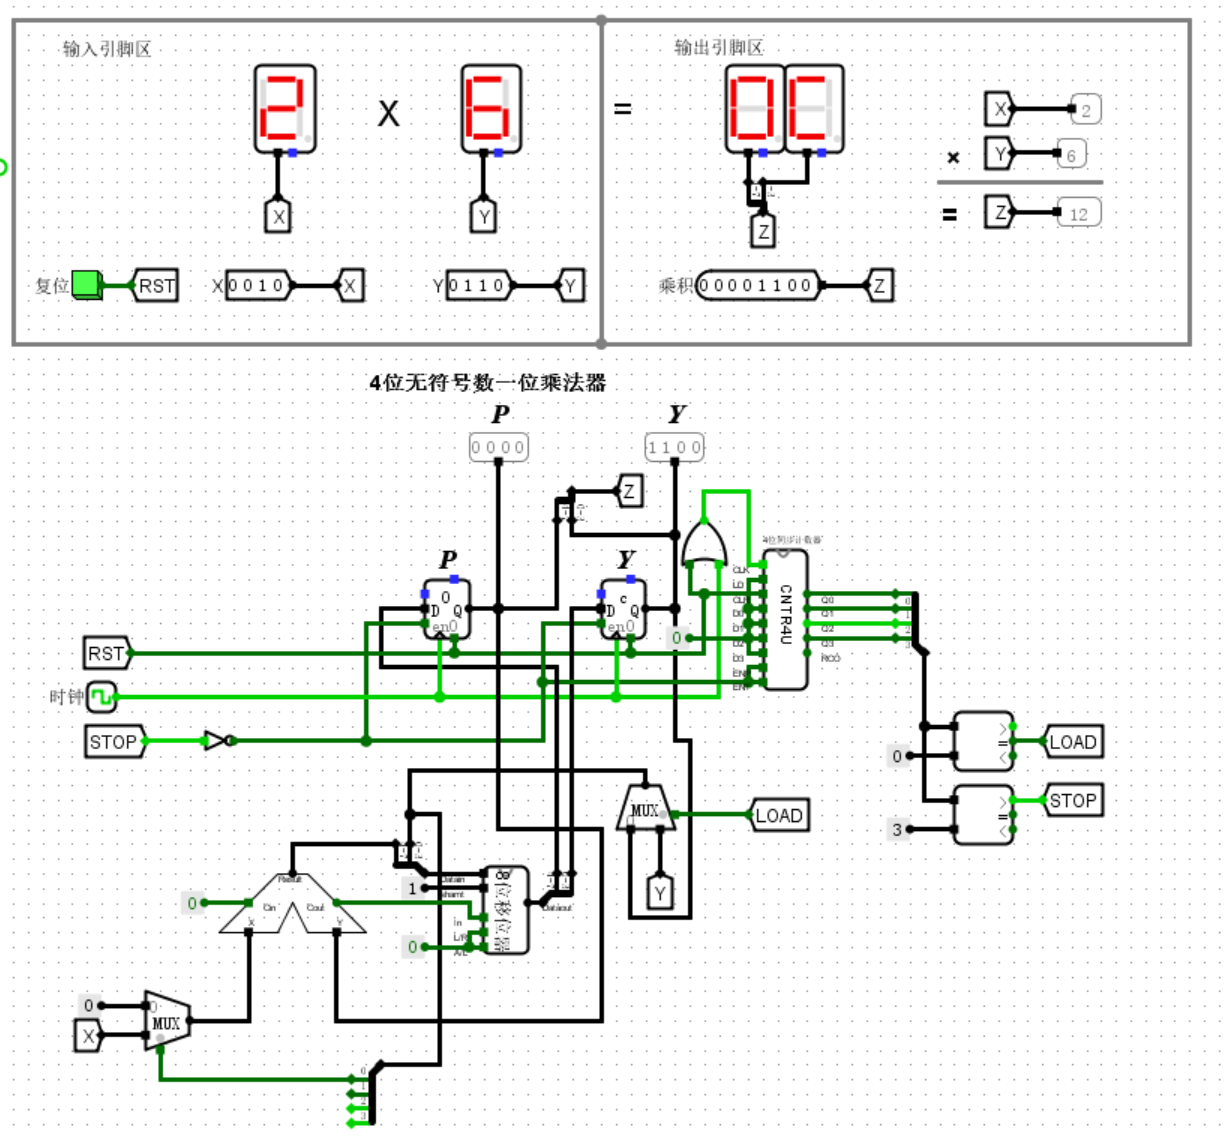
\includegraphics[width=0.7\textwidth]{4.5.3.png}
    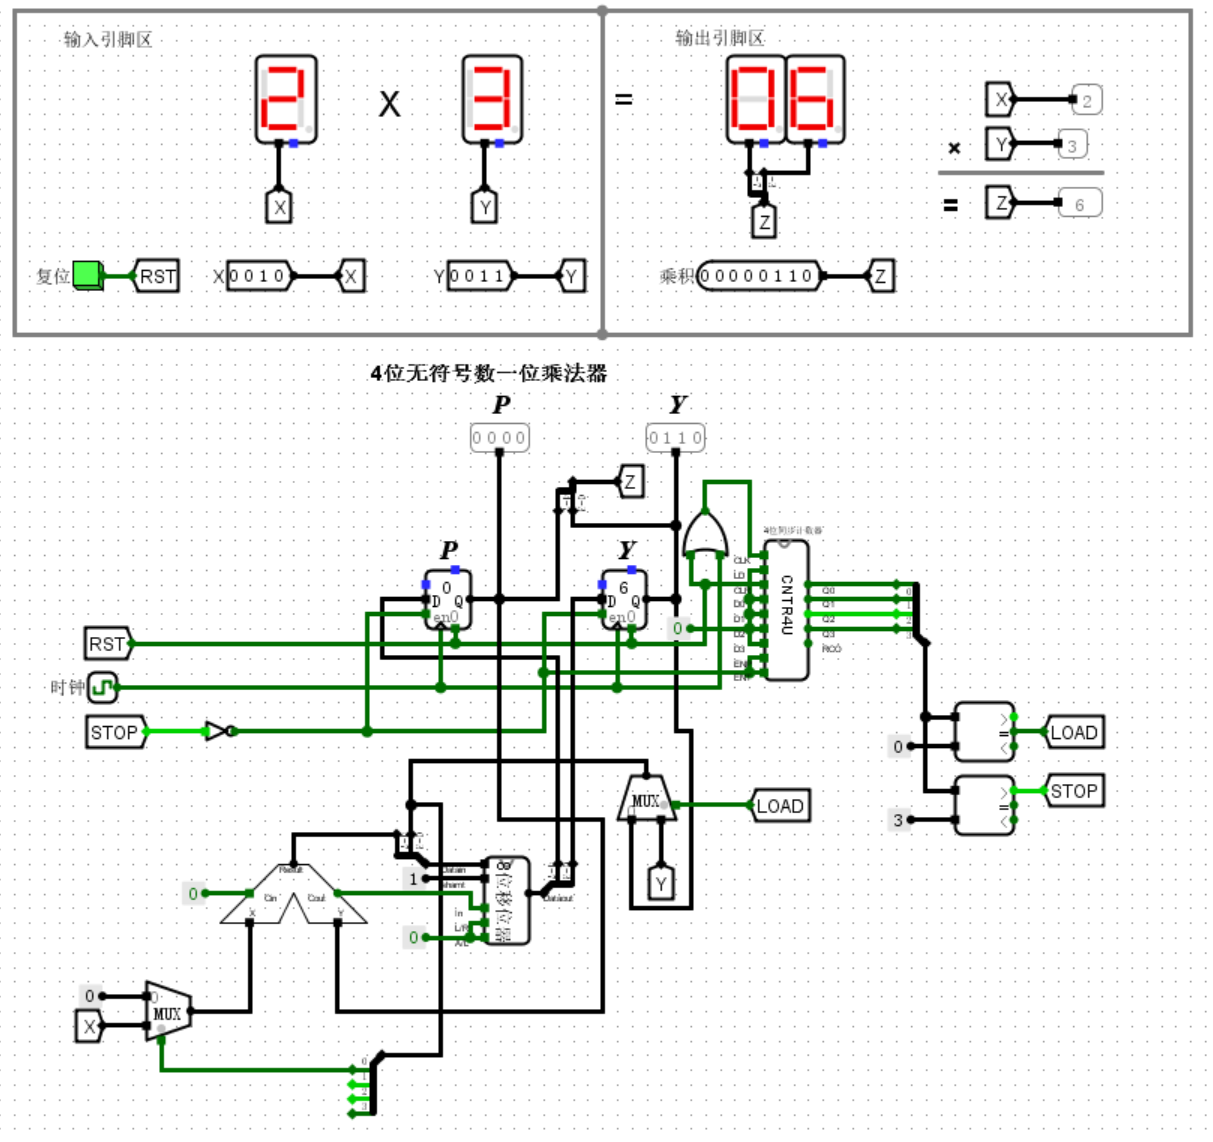
\includegraphics[width=0.7\textwidth]{4.5.4.png}
    \caption{4位无符号数乘法器仿真测试图}
    \end{figure}

    复位后经过三个时钟周期可算出乘法结果。

    \subsubsection{错误现象及分析}
    在完成实验的过程中,没有遇到任何错误。

    \subsection{寄存器堆实验}
    \subsubsection{整体方案设计}
    \begin{figure}[H]
    \centering
    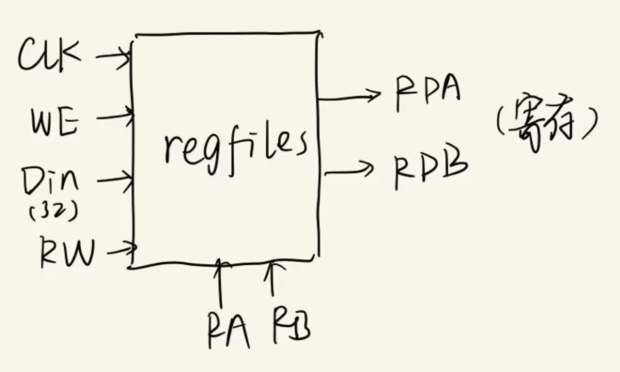
\includegraphics[width=0.8\textwidth]{5.1.png}
    \caption{寄存器堆整体方案设计}
    \end{figure}
    
    \subsubsection{顶层模块设计}
    实验电路较为简单,不需要顶层模块设计图。
    
    \subsubsection{引脚作用}
    \begin{table}[H]    
    \centering
    \begin{tabular}{|c|c|}
        \hline
        CLK & 时钟信号 \\ \hline
        RA,RB & 读取数据地址 \\ \hline
        WE & 写使能 \\ \hline
        DIN & 输入引脚 \\ \hline
        RDA,RDB  & 输出引脚 \\ \hline
    \end{tabular}
    \caption{寄存器堆引脚作用}
    \end{table}

    \subsubsection{原理图和电路图}
    \begin{figure}[H]
    \centering
    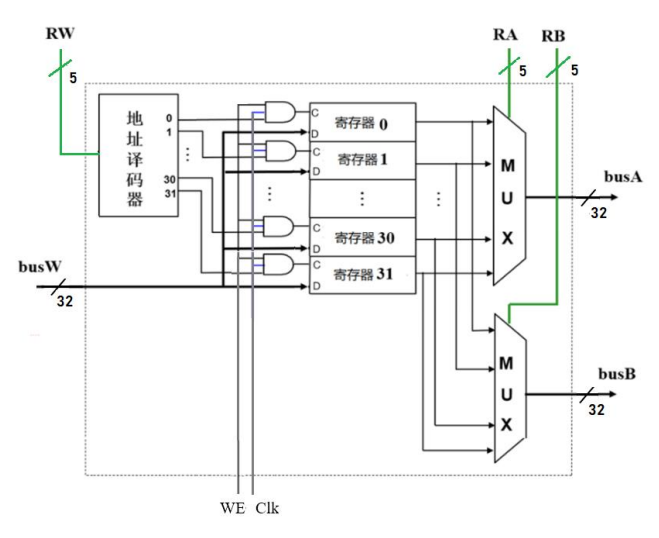
\includegraphics[width=0.8\textwidth]{5.4.1.png}
    \caption{寄存器堆原理图}
    \end{figure}

    \begin{figure}[H]
    \centering
    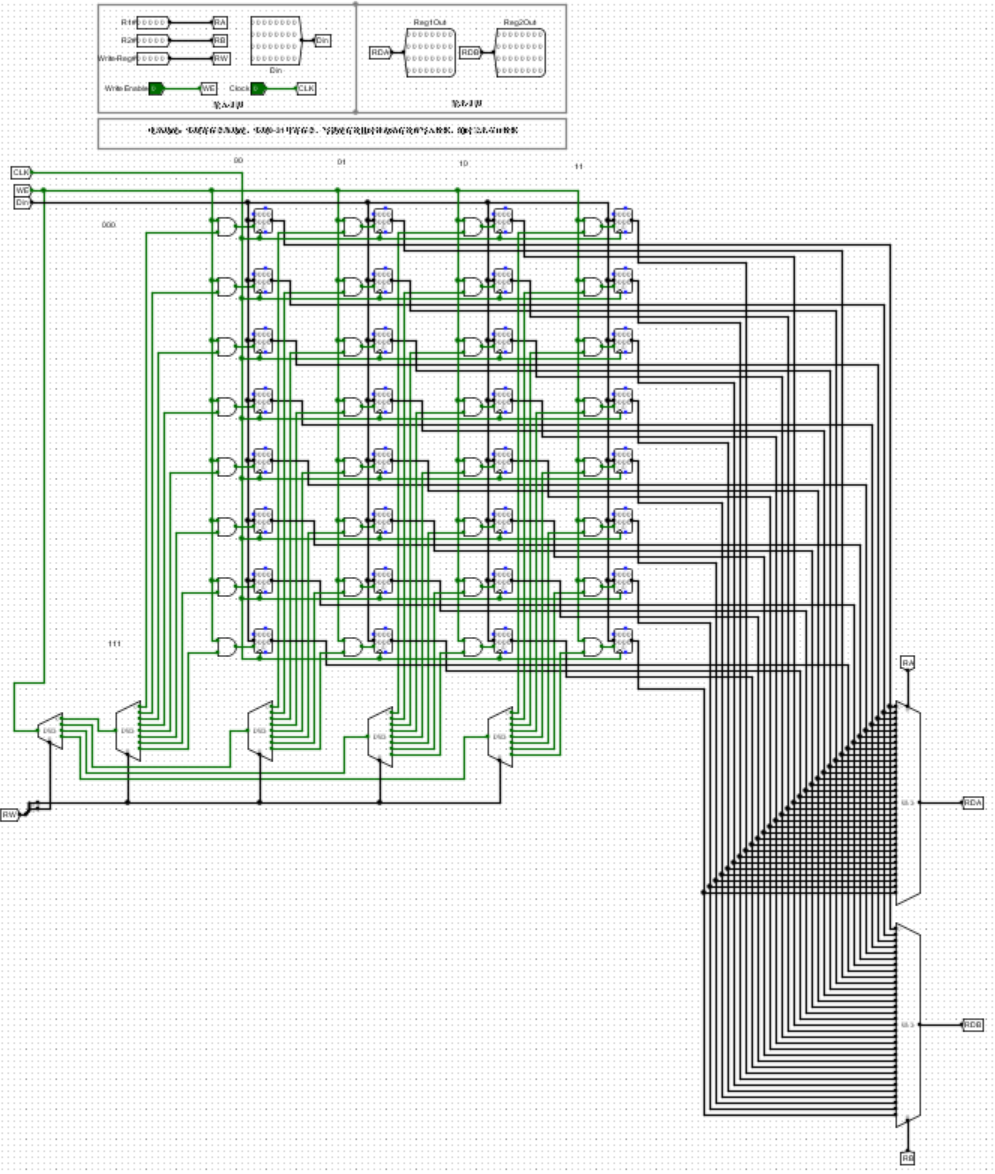
\includegraphics[width=0.8\textwidth]{5.4.2.png}
    \caption{寄存器堆电路图}
    \end{figure}

    \subsubsection{仿真测试图}
    \begin{figure}[H]
    \centering
    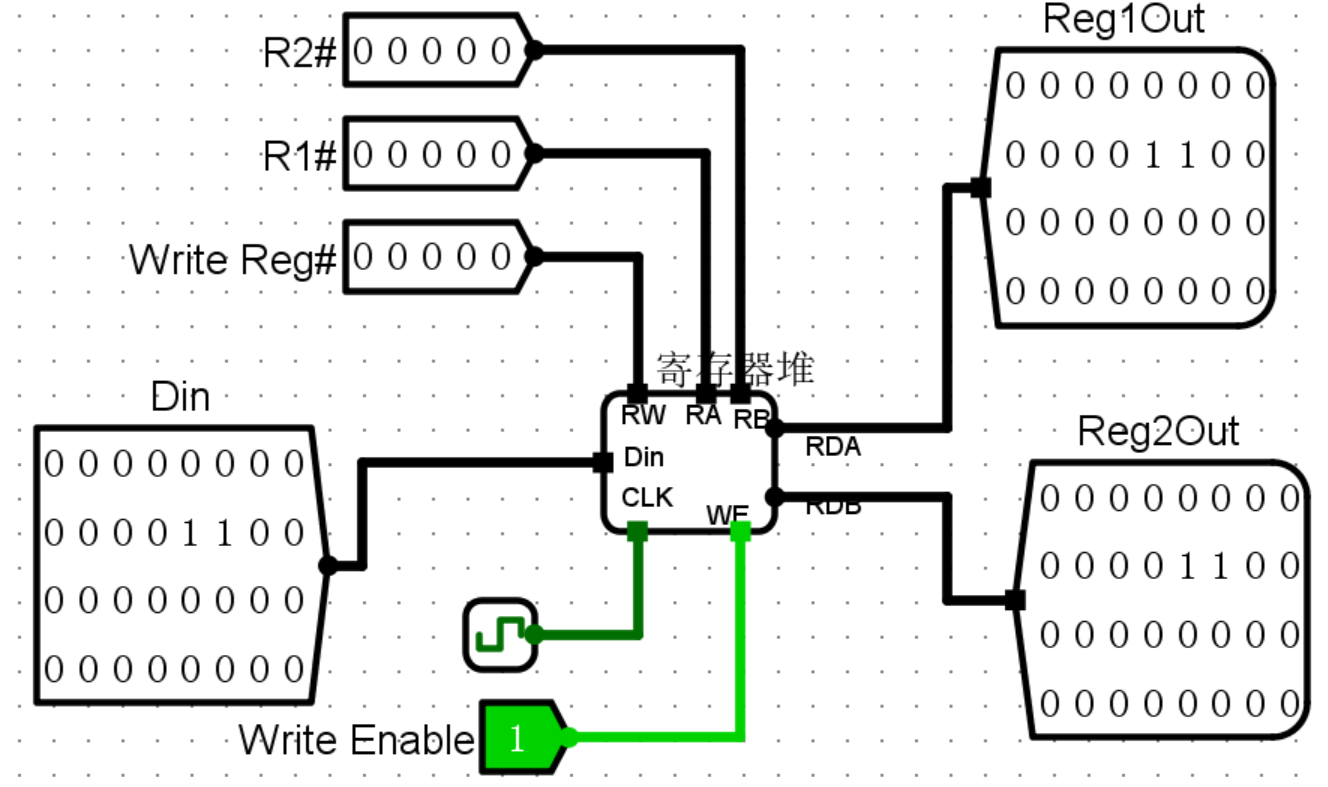
\includegraphics[width=0.8\textwidth]{5.5.1.png}
    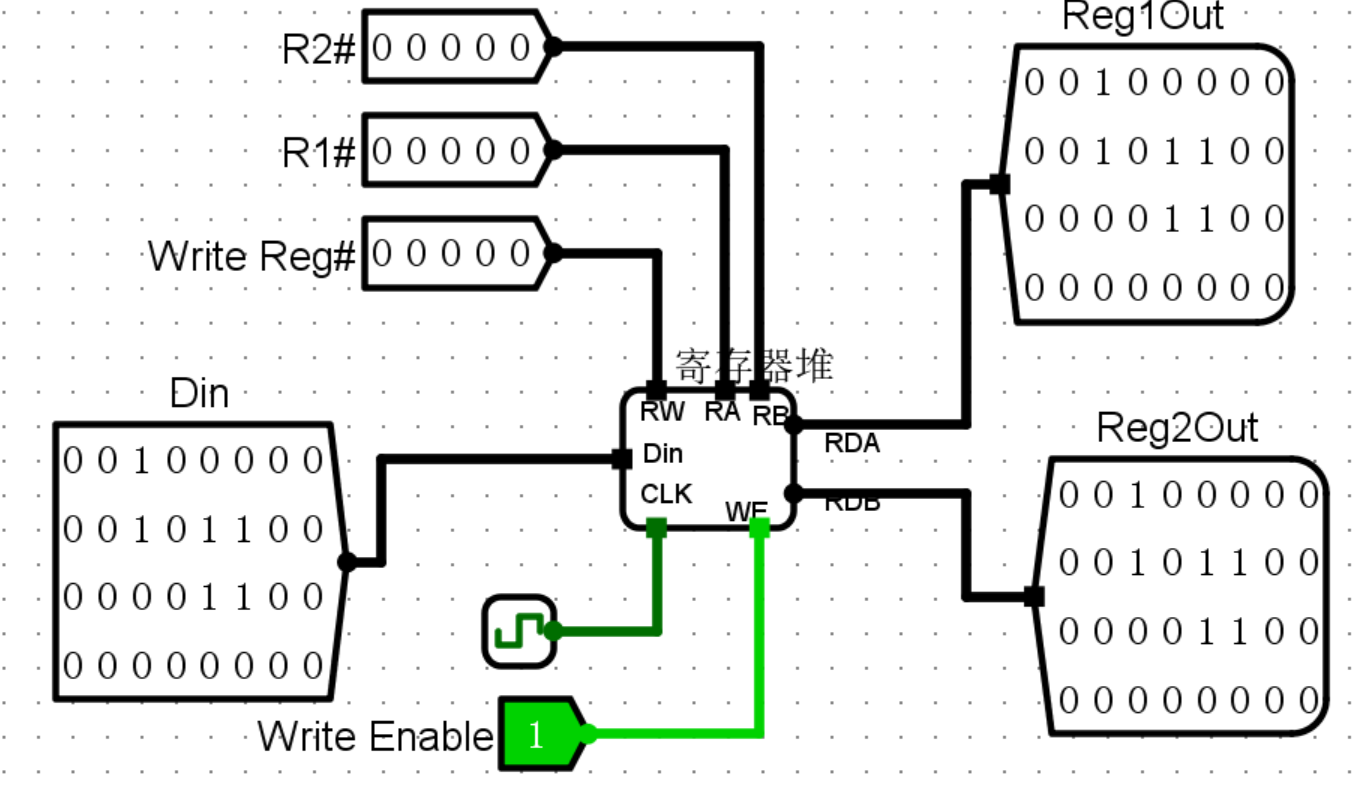
\includegraphics[width=0.8\textwidth]{5.5.2.png}
    \caption{寄存器堆仿真测试图}
    \end{figure}

    \subsubsection{错误现象及分析}  
    在完成实验的过程中,没有遇到任何错误。



    
    
    \section{思考题}

    \subsection{在数字时钟实验中,如果需要增加闹钟功能,电路中需要如何修改?}
    使用比较器后连接蜂鸣使能,比较器的左端为闹铃设置的时间点即可。
    \begin{figure}[H]
        \centering
        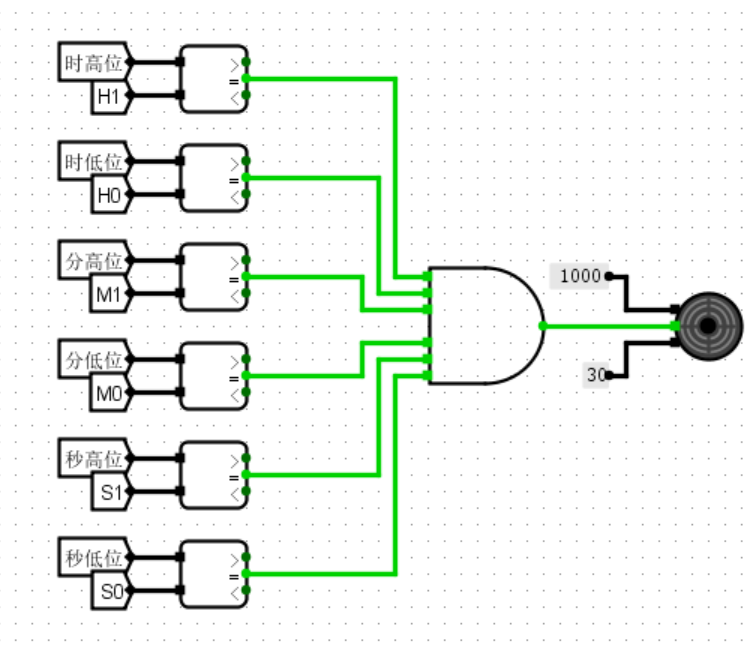
\includegraphics[width=0.8\textwidth]{6.1.png}
        \caption{闹钟功能电路图}
    \end{figure}

    \subsection{如何修改 4 位无符号数乘法器电路,使其实现 4 位 Booth 乘法器的功能?}
    将原来的乘法器改为 Booth 乘法器的对x每两位判断一次进行运算即可,为实现以上操作,在LOAD和x输入间加上D触发器,每一个时钟周期进行一次运算。
    \begin{figure}[H]
        \centering
        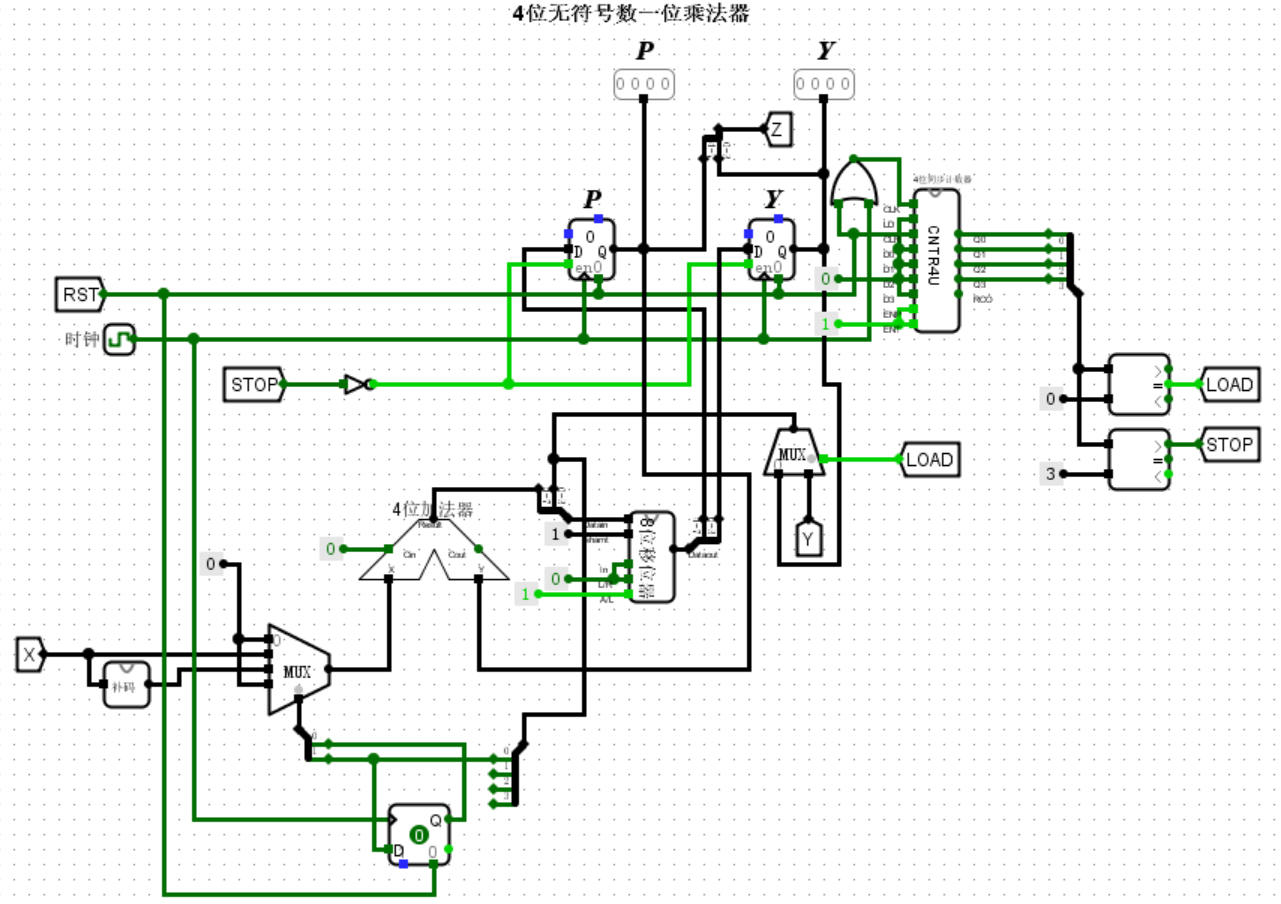
\includegraphics[width=0.8\textwidth]{7.1.png}
        \caption{4位Booth乘法器电路图}
    \end{figure}

    \subsection{如何实现 4 位无符号数除法器?}
    采用恢复余数法,当余数为负数(即最高为1时,为负数)时,需要加上除数,将其恢复成原来的余数,而商值的大小是通过比较被除数和除数的绝对值的大小确定的。
    将加法器的Cout连接上每次执行比较运算的MUX,若差值为正数,则将Cout置为1,否则置为0,若Cout为1,则将商值加1,将x置为差值;若Cout为0,则将商值置为0,将x置为原来的被除数(保持不变)。
    \begin{figure}[H]
        \centering
        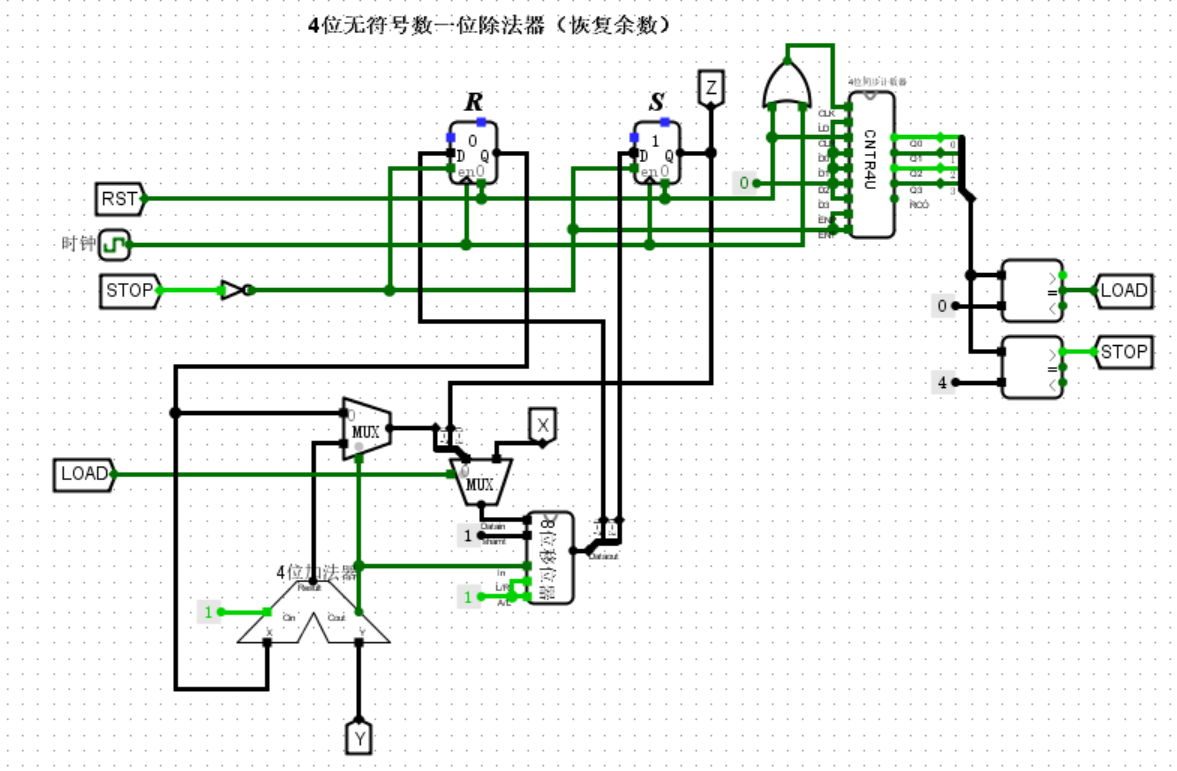
\includegraphics[width=0.8\textwidth]{8.1.png}
        \caption{4位无符号数除法器电路图}
    \end{figure}
\end{document}